% Created by tikzDevice version 0.12.5 on 2023-10-26 18:47:52
% !TEX encoding = UTF-8 Unicode
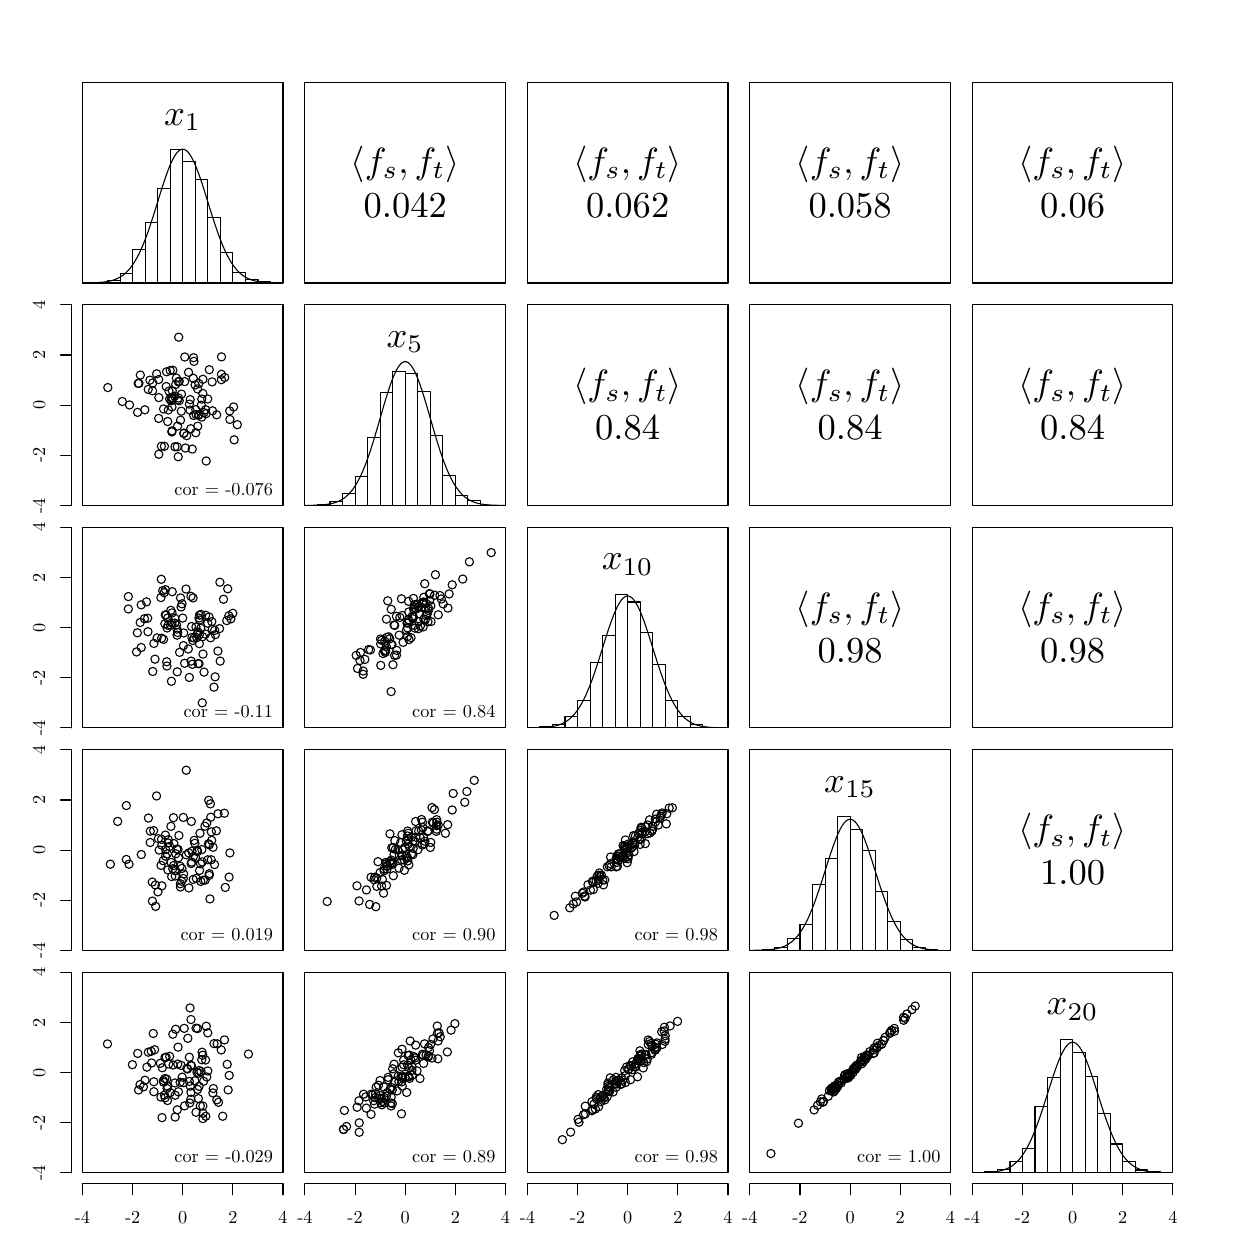
\begin{tikzpicture}[x=1pt,y=1pt]
\definecolor{fillColor}{RGB}{255,255,255}
\path[use as bounding box,fill=fillColor,fill opacity=0.00] (0,0) rectangle (433.62,433.62);
\begin{scope}
\path[clip] (  0.00,  0.00) rectangle (433.62,433.62);
\definecolor{drawColor}{RGB}{0,0,0}

\path[draw=drawColor,line width= 0.4pt,line join=round,line cap=round] ( 19.80,341.35) --
	( 92.27,341.35) --
	( 92.27,413.82) --
	( 19.80,413.82) --
	cycle;
\end{scope}
\begin{scope}
\path[clip] ( 19.80,341.35) rectangle ( 92.27,413.82);
\definecolor{drawColor}{RGB}{0,0,0}

\path[draw=drawColor,line width= 0.4pt,line join=round,line cap=round] ( 19.80,341.35) rectangle ( 24.33,341.43);

\path[draw=drawColor,line width= 0.4pt,line join=round,line cap=round] ( 24.33,341.35) rectangle ( 28.86,341.43);

\path[draw=drawColor,line width= 0.4pt,line join=round,line cap=round] ( 28.86,341.35) rectangle ( 33.39,342.32);

\path[draw=drawColor,line width= 0.4pt,line join=round,line cap=round] ( 33.39,341.35) rectangle ( 37.92,344.91);

\path[draw=drawColor,line width= 0.4pt,line join=round,line cap=round] ( 37.92,341.35) rectangle ( 42.45,353.47);

\path[draw=drawColor,line width= 0.4pt,line join=round,line cap=round] ( 42.45,341.35) rectangle ( 46.98,363.17);

\path[draw=drawColor,line width= 0.4pt,line join=round,line cap=round] ( 46.98,341.35) rectangle ( 51.50,375.53);

\path[draw=drawColor,line width= 0.4pt,line join=round,line cap=round] ( 51.50,341.35) rectangle ( 56.03,389.66);

\path[draw=drawColor,line width= 0.4pt,line join=round,line cap=round] ( 56.03,341.35) rectangle ( 60.56,385.38);

\path[draw=drawColor,line width= 0.4pt,line join=round,line cap=round] ( 60.56,341.35) rectangle ( 65.09,378.68);

\path[draw=drawColor,line width= 0.4pt,line join=round,line cap=round] ( 65.09,341.35) rectangle ( 69.62,364.94);

\path[draw=drawColor,line width= 0.4pt,line join=round,line cap=round] ( 69.62,341.35) rectangle ( 74.15,352.34);

\path[draw=drawColor,line width= 0.4pt,line join=round,line cap=round] ( 74.15,341.35) rectangle ( 78.68,345.07);

\path[draw=drawColor,line width= 0.4pt,line join=round,line cap=round] ( 78.68,341.35) rectangle ( 83.21,342.56);

\path[draw=drawColor,line width= 0.4pt,line join=round,line cap=round] ( 83.21,341.35) rectangle ( 87.74,341.76);

\path[draw=drawColor,line width= 0.4pt,line join=round,line cap=round] ( 19.80,341.37) --
	( 20.48,341.37) --
	( 21.16,341.38) --
	( 21.84,341.39) --
	( 22.52,341.40) --
	( 23.20,341.42) --
	( 23.88,341.44) --
	( 24.56,341.47) --
	( 25.24,341.50) --
	( 25.91,341.54) --
	( 26.59,341.60) --
	( 27.27,341.66) --
	( 27.95,341.75) --
	( 28.63,341.85) --
	( 29.31,341.98) --
	( 29.99,342.13) --
	( 30.67,342.31) --
	( 31.35,342.53) --
	( 32.03,342.80) --
	( 32.71,343.11) --
	( 33.39,343.48) --
	( 34.07,343.91) --
	( 34.75,344.41) --
	( 35.43,344.99) --
	( 36.11,345.65) --
	( 36.78,346.41) --
	( 37.46,347.26) --
	( 38.14,348.23) --
	( 38.82,349.30) --
	( 39.50,350.50) --
	( 40.18,351.81) --
	( 40.86,353.24) --
	( 41.54,354.79) --
	( 42.22,356.47) --
	( 42.90,358.25) --
	( 43.58,360.14) --
	( 44.26,362.12) --
	( 44.94,364.18) --
	( 45.62,366.31) --
	( 46.30,368.48) --
	( 46.98,370.67) --
	( 47.65,372.87) --
	( 48.33,375.04) --
	( 49.01,377.16) --
	( 49.69,379.19) --
	( 50.37,381.12) --
	( 51.05,382.91) --
	( 51.73,384.54) --
	( 52.41,385.98) --
	( 53.09,387.21) --
	( 53.77,388.21) --
	( 54.45,388.96) --
	( 55.13,389.46) --
	( 55.81,389.68) --
	( 56.49,389.64) --
	( 57.17,389.32) --
	( 57.85,388.74) --
	( 58.53,387.90) --
	( 59.20,386.83) --
	( 59.88,385.52) --
	( 60.56,384.02) --
	( 61.24,382.33) --
	( 61.92,380.49) --
	( 62.60,378.52) --
	( 63.28,376.46) --
	( 63.96,374.32) --
	( 64.64,372.14) --
	( 65.32,369.94) --
	( 66.00,367.75) --
	( 66.68,365.59) --
	( 67.36,363.49) --
	( 68.04,361.45) --
	( 68.72,359.50) --
	( 69.40,357.64) --
	( 70.07,355.90) --
	( 70.75,354.26) --
	( 71.43,352.75) --
	( 72.11,351.36) --
	( 72.79,350.09) --
	( 73.47,348.93) --
	( 74.15,347.89) --
	( 74.83,346.97) --
	( 75.51,346.14) --
	( 76.19,345.42) --
	( 76.87,344.78) --
	( 77.55,344.23) --
	( 78.23,343.76) --
	( 78.91,343.35) --
	( 79.59,343.00) --
	( 80.27,342.70) --
	( 80.94,342.45) --
	( 81.62,342.25) --
	( 82.30,342.07) --
	( 82.98,341.93) --
	( 83.66,341.81) --
	( 84.34,341.72) --
	( 85.02,341.64) --
	( 85.70,341.58) --
	( 86.38,341.53) --
	( 87.06,341.49) --
	( 87.74,341.46);
\end{scope}
\begin{scope}
\path[clip] (  0.00,  0.00) rectangle (433.62,433.62);
\definecolor{drawColor}{RGB}{0,0,0}

\path[draw=drawColor,line width= 0.4pt,line join=round,line cap=round] ( 19.80, 15.84) -- ( 92.27, 15.84);

\path[draw=drawColor,line width= 0.4pt,line join=round,line cap=round] ( 19.80, 15.84) -- ( 19.80, 11.88);

\path[draw=drawColor,line width= 0.4pt,line join=round,line cap=round] ( 37.92, 15.84) -- ( 37.92, 11.88);

\path[draw=drawColor,line width= 0.4pt,line join=round,line cap=round] ( 56.03, 15.84) -- ( 56.03, 11.88);

\path[draw=drawColor,line width= 0.4pt,line join=round,line cap=round] ( 74.15, 15.84) -- ( 74.15, 11.88);

\path[draw=drawColor,line width= 0.4pt,line join=round,line cap=round] ( 92.27, 15.84) -- ( 92.27, 11.88);

\node[text=drawColor,anchor=base,inner sep=0pt, outer sep=0pt, scale=  0.66] at ( 19.80,  1.58) {-4};

\node[text=drawColor,anchor=base,inner sep=0pt, outer sep=0pt, scale=  0.66] at ( 37.92,  1.58) {-2};

\node[text=drawColor,anchor=base,inner sep=0pt, outer sep=0pt, scale=  0.66] at ( 56.03,  1.58) {0};

\node[text=drawColor,anchor=base,inner sep=0pt, outer sep=0pt, scale=  0.66] at ( 74.15,  1.58) {2};

\node[text=drawColor,anchor=base,inner sep=0pt, outer sep=0pt, scale=  0.66] at ( 92.27,  1.58) {4};
\end{scope}
\begin{scope}
\path[clip] ( 19.80,341.35) rectangle ( 92.27,413.82);
\definecolor{drawColor}{RGB}{0,0,0}

\node[text=drawColor,anchor=base,inner sep=0pt, outer sep=0pt, scale=  1.32] at ( 56.03,398.44) {$x_{1}$};
\end{scope}
\begin{scope}
\path[clip] (  0.00,  0.00) rectangle (433.62,433.62);
\definecolor{drawColor}{RGB}{0,0,0}

\path[draw=drawColor,line width= 0.4pt,line join=round,line cap=round] ( 19.80,260.96) --
	( 92.27,260.96) --
	( 92.27,333.43) --
	( 19.80,333.43) --
	cycle;
\end{scope}
\begin{scope}
\path[clip] ( 19.80,260.96) rectangle ( 92.27,333.43);
\definecolor{drawColor}{RGB}{0,0,0}

\path[draw=drawColor,line width= 0.4pt,line join=round,line cap=round] ( 53.73,306.99) circle (  1.49);

\path[draw=drawColor,line width= 0.4pt,line join=round,line cap=round] ( 65.63,310.03) circle (  1.49);

\path[draw=drawColor,line width= 0.4pt,line join=round,line cap=round] ( 54.76,305.84) circle (  1.49);

\path[draw=drawColor,line width= 0.4pt,line join=round,line cap=round] ( 59.94,314.36) circle (  1.49);

\path[draw=drawColor,line width= 0.4pt,line join=round,line cap=round] ( 47.38,279.46) circle (  1.49);

\path[draw=drawColor,line width= 0.4pt,line join=round,line cap=round] ( 71.20,307.21) circle (  1.49);

\path[draw=drawColor,line width= 0.4pt,line join=round,line cap=round] ( 64.31,295.58) circle (  1.49);

\path[draw=drawColor,line width= 0.4pt,line join=round,line cap=round] ( 44.16,306.25) circle (  1.49);

\path[draw=drawColor,line width= 0.4pt,line join=round,line cap=round] ( 49.41,282.36) circle (  1.49);

\path[draw=drawColor,line width= 0.4pt,line join=round,line cap=round] ( 54.18,289.66) circle (  1.49);

\path[draw=drawColor,line width= 0.4pt,line join=round,line cap=round] ( 62.74,297.18) circle (  1.49);

\path[draw=drawColor,line width= 0.4pt,line join=round,line cap=round] ( 62.91,299.40) circle (  1.49);

\path[draw=drawColor,line width= 0.4pt,line join=round,line cap=round] ( 58.13,309.09) circle (  1.49);

\path[draw=drawColor,line width= 0.4pt,line join=round,line cap=round] ( 57.46,286.19) circle (  1.49);

\path[draw=drawColor,line width= 0.4pt,line join=round,line cap=round] ( 46.59,308.53) circle (  1.49);

\path[draw=drawColor,line width= 0.4pt,line join=round,line cap=round] ( 66.79,295.16) circle (  1.49);

\path[draw=drawColor,line width= 0.4pt,line join=round,line cap=round] ( 60.51,304.51) circle (  1.49);

\path[draw=drawColor,line width= 0.4pt,line join=round,line cap=round] ( 28.96,303.57) circle (  1.49);

\path[draw=drawColor,line width= 0.4pt,line join=round,line cap=round] ( 53.11,300.45) circle (  1.49);

\path[draw=drawColor,line width= 0.4pt,line join=round,line cap=round] ( 51.30,299.45) circle (  1.49);

\path[draw=drawColor,line width= 0.4pt,line join=round,line cap=round] ( 60.09,313.03) circle (  1.49);

\path[draw=drawColor,line width= 0.4pt,line join=round,line cap=round] ( 51.50,309.73) circle (  1.49);

\path[draw=drawColor,line width= 0.4pt,line join=round,line cap=round] ( 70.00,308.36) circle (  1.49);

\path[draw=drawColor,line width= 0.4pt,line join=round,line cap=round] ( 52.36,299.93) circle (  1.49);

\path[draw=drawColor,line width= 0.4pt,line join=round,line cap=round] ( 61.70,293.54) circle (  1.49);

\path[draw=drawColor,line width= 0.4pt,line join=round,line cap=round] ( 52.46,309.82) circle (  1.49);

\path[draw=drawColor,line width= 0.4pt,line join=round,line cap=round] ( 45.18,305.22) circle (  1.49);

\path[draw=drawColor,line width= 0.4pt,line join=round,line cap=round] ( 52.21,299.35) circle (  1.49);

\path[draw=drawColor,line width= 0.4pt,line join=round,line cap=round] ( 63.30,301.43) circle (  1.49);

\path[draw=drawColor,line width= 0.4pt,line join=round,line cap=round] ( 54.18,299.12) circle (  1.49);

\path[draw=drawColor,line width= 0.4pt,line join=round,line cap=round] ( 51.82,298.79) circle (  1.49);

\path[draw=drawColor,line width= 0.4pt,line join=round,line cap=round] ( 52.09,287.54) circle (  1.49);

\path[draw=drawColor,line width= 0.4pt,line join=round,line cap=round] ( 39.72,294.61) circle (  1.49);

\path[draw=drawColor,line width= 0.4pt,line join=round,line cap=round] ( 58.73,299.21) circle (  1.49);

\path[draw=drawColor,line width= 0.4pt,line join=round,line cap=round] ( 73.07,292.05) circle (  1.49);

\path[draw=drawColor,line width= 0.4pt,line join=round,line cap=round] ( 54.51,299.80) circle (  1.49);

\path[draw=drawColor,line width= 0.4pt,line join=round,line cap=round] ( 47.41,299.95) circle (  1.49);

\path[draw=drawColor,line width= 0.4pt,line join=round,line cap=round] ( 51.04,302.29) circle (  1.49);

\path[draw=drawColor,line width= 0.4pt,line join=round,line cap=round] ( 56.73,305.72) circle (  1.49);

\path[draw=drawColor,line width= 0.4pt,line join=round,line cap=round] ( 56.47,287.13) circle (  1.49);

\path[draw=drawColor,line width= 0.4pt,line join=round,line cap=round] ( 42.33,295.53) circle (  1.49);

\path[draw=drawColor,line width= 0.4pt,line join=round,line cap=round] ( 58.43,297.59) circle (  1.49);

\path[draw=drawColor,line width= 0.4pt,line join=round,line cap=round] ( 58.65,295.42) circle (  1.49);

\path[draw=drawColor,line width= 0.4pt,line join=round,line cap=round] ( 53.22,282.16) circle (  1.49);

\path[draw=drawColor,line width= 0.4pt,line join=round,line cap=round] ( 55.23,291.79) circle (  1.49);

\path[draw=drawColor,line width= 0.4pt,line join=round,line cap=round] ( 49.09,295.85) circle (  1.49);

\path[draw=drawColor,line width= 0.4pt,line join=round,line cap=round] ( 34.20,298.53) circle (  1.49);

\path[draw=drawColor,line width= 0.4pt,line join=round,line cap=round] ( 74.41,296.58) circle (  1.49);

\path[draw=drawColor,line width= 0.4pt,line join=round,line cap=round] ( 50.84,295.50) circle (  1.49);

\path[draw=drawColor,line width= 0.4pt,line join=round,line cap=round] ( 59.47,281.34) circle (  1.49);

\path[draw=drawColor,line width= 0.4pt,line join=round,line cap=round] ( 56.41,286.96) circle (  1.49);

\path[draw=drawColor,line width= 0.4pt,line join=round,line cap=round] ( 60.73,287.25) circle (  1.49);

\path[draw=drawColor,line width= 0.4pt,line join=round,line cap=round] ( 64.47,294.15) circle (  1.49);

\path[draw=drawColor,line width= 0.4pt,line join=round,line cap=round] ( 62.90,292.90) circle (  1.49);

\path[draw=drawColor,line width= 0.4pt,line join=round,line cap=round] ( 70.01,306.42) circle (  1.49);

\path[draw=drawColor,line width= 0.4pt,line join=round,line cap=round] ( 59.83,306.93) circle (  1.49);

\path[draw=drawColor,line width= 0.4pt,line join=round,line cap=round] ( 39.92,305.07) circle (  1.49);

\path[draw=drawColor,line width= 0.4pt,line join=round,line cap=round] ( 40.71,308.09) circle (  1.49);

\path[draw=drawColor,line width= 0.4pt,line join=round,line cap=round] ( 59.98,293.48) circle (  1.49);

\path[draw=drawColor,line width= 0.4pt,line join=round,line cap=round] ( 47.35,306.47) circle (  1.49);

\path[draw=drawColor,line width= 0.4pt,line join=round,line cap=round] ( 60.74,295.60) circle (  1.49);

\path[draw=drawColor,line width= 0.4pt,line join=round,line cap=round] ( 43.56,302.91) circle (  1.49);

\path[draw=drawColor,line width= 0.4pt,line join=round,line cap=round] ( 40.20,305.10) circle (  1.49);

\path[draw=drawColor,line width= 0.4pt,line join=round,line cap=round] ( 54.06,282.17) circle (  1.49);

\path[draw=drawColor,line width= 0.4pt,line join=round,line cap=round] ( 61.89,293.80) circle (  1.49);

\path[draw=drawColor,line width= 0.4pt,line join=round,line cap=round] ( 52.25,302.42) circle (  1.49);

\path[draw=drawColor,line width= 0.4pt,line join=round,line cap=round] ( 66.65,305.62) circle (  1.49);

\path[draw=drawColor,line width= 0.4pt,line join=round,line cap=round] ( 48.32,282.37) circle (  1.49);

\path[draw=drawColor,line width= 0.4pt,line join=round,line cap=round] ( 55.58,301.19) circle (  1.49);

\path[draw=drawColor,line width= 0.4pt,line join=round,line cap=round] ( 50.06,303.94) circle (  1.49);

\path[draw=drawColor,line width= 0.4pt,line join=round,line cap=round] ( 52.06,299.95) circle (  1.49);

\path[draw=drawColor,line width= 0.4pt,line join=round,line cap=round] ( 54.39,278.58) circle (  1.49);

\path[draw=drawColor,line width= 0.4pt,line join=round,line cap=round] ( 60.88,293.81) circle (  1.49);

\path[draw=drawColor,line width= 0.4pt,line join=round,line cap=round] ( 54.78,298.84) circle (  1.49);

\path[draw=drawColor,line width= 0.4pt,line join=round,line cap=round] ( 63.68,294.53) circle (  1.49);

\path[draw=drawColor,line width= 0.4pt,line join=round,line cap=round] ( 56.77,314.61) circle (  1.49);

\path[draw=drawColor,line width= 0.4pt,line join=round,line cap=round] ( 36.79,297.29) circle (  1.49);

\path[draw=drawColor,line width= 0.4pt,line join=round,line cap=round] ( 61.38,303.09) circle (  1.49);

\path[draw=drawColor,line width= 0.4pt,line join=round,line cap=round] ( 65.04,299.44) circle (  1.49);

\path[draw=drawColor,line width= 0.4pt,line join=round,line cap=round] ( 54.48,305.62) circle (  1.49);

\path[draw=drawColor,line width= 0.4pt,line join=round,line cap=round] ( 53.50,304.67) circle (  1.49);

\path[draw=drawColor,line width= 0.4pt,line join=round,line cap=round] ( 63.31,306.55) circle (  1.49);

\path[draw=drawColor,line width= 0.4pt,line join=round,line cap=round] ( 52.14,296.57) circle (  1.49);

\path[draw=drawColor,line width= 0.4pt,line join=round,line cap=round] ( 57.01,281.71) circle (  1.49);

\path[draw=drawColor,line width= 0.4pt,line join=round,line cap=round] ( 54.58,321.77) circle (  1.49);

\path[draw=drawColor,line width= 0.4pt,line join=round,line cap=round] ( 61.84,305.05) circle (  1.49);

\path[draw=drawColor,line width= 0.4pt,line join=round,line cap=round] ( 58.94,288.70) circle (  1.49);

\path[draw=drawColor,line width= 0.4pt,line join=round,line cap=round] ( 74.61,284.68) circle (  1.49);

\path[draw=drawColor,line width= 0.4pt,line join=round,line cap=round] ( 55.51,295.04) circle (  1.49);

\path[draw=drawColor,line width= 0.4pt,line join=round,line cap=round] ( 70.04,314.66) circle (  1.49);

\path[draw=drawColor,line width= 0.4pt,line join=round,line cap=round] ( 50.59,291.29) circle (  1.49);

\path[draw=drawColor,line width= 0.4pt,line join=round,line cap=round] ( 73.00,295.13) circle (  1.49);

\path[draw=drawColor,line width= 0.4pt,line join=round,line cap=round] ( 64.50,277.04) circle (  1.49);

\path[draw=drawColor,line width= 0.4pt,line join=round,line cap=round] ( 52.18,287.92) circle (  1.49);

\path[draw=drawColor,line width= 0.4pt,line join=round,line cap=round] ( 50.20,309.27) circle (  1.49);

\path[draw=drawColor,line width= 0.4pt,line join=round,line cap=round] ( 68.28,293.72) circle (  1.49);

\path[draw=drawColor,line width= 0.4pt,line join=round,line cap=round] ( 45.13,302.38) circle (  1.49);

\path[draw=drawColor,line width= 0.4pt,line join=round,line cap=round] ( 47.34,292.42) circle (  1.49);

\path[draw=drawColor,line width= 0.4pt,line join=round,line cap=round] ( 75.75,290.16) circle (  1.49);

\path[draw=drawColor,line width= 0.4pt,line join=round,line cap=round] ( 61.46,289.62) circle (  1.49);

\node[text=drawColor,anchor=base east,inner sep=0pt, outer sep=0pt, scale=  0.66] at ( 88.64,264.59) {cor = -0.076};
\end{scope}
\begin{scope}
\path[clip] (  0.00,  0.00) rectangle (433.62,433.62);
\definecolor{drawColor}{RGB}{0,0,0}

\path[draw=drawColor,line width= 0.4pt,line join=round,line cap=round] ( 15.84,260.96) -- ( 15.84,333.43);

\path[draw=drawColor,line width= 0.4pt,line join=round,line cap=round] ( 15.84,260.96) -- ( 11.88,260.96);

\path[draw=drawColor,line width= 0.4pt,line join=round,line cap=round] ( 15.84,279.08) -- ( 11.88,279.08);

\path[draw=drawColor,line width= 0.4pt,line join=round,line cap=round] ( 15.84,297.20) -- ( 11.88,297.20);

\path[draw=drawColor,line width= 0.4pt,line join=round,line cap=round] ( 15.84,315.32) -- ( 11.88,315.32);

\path[draw=drawColor,line width= 0.4pt,line join=round,line cap=round] ( 15.84,333.43) -- ( 11.88,333.43);

\node[text=drawColor,rotate= 90.00,anchor=base,inner sep=0pt, outer sep=0pt, scale=  0.66] at (  6.34,260.96) {-4};

\node[text=drawColor,rotate= 90.00,anchor=base,inner sep=0pt, outer sep=0pt, scale=  0.66] at (  6.34,279.08) {-2};

\node[text=drawColor,rotate= 90.00,anchor=base,inner sep=0pt, outer sep=0pt, scale=  0.66] at (  6.34,297.20) {0};

\node[text=drawColor,rotate= 90.00,anchor=base,inner sep=0pt, outer sep=0pt, scale=  0.66] at (  6.34,315.32) {2};

\node[text=drawColor,rotate= 90.00,anchor=base,inner sep=0pt, outer sep=0pt, scale=  0.66] at (  6.34,333.43) {4};
\end{scope}
\begin{scope}
\path[clip] (  0.00,  0.00) rectangle (433.62,433.62);
\definecolor{drawColor}{RGB}{0,0,0}

\path[draw=drawColor,line width= 0.4pt,line join=round,line cap=round] ( 19.80,180.58) --
	( 92.27,180.58) --
	( 92.27,253.04) --
	( 19.80,253.04) --
	cycle;
\end{scope}
\begin{scope}
\path[clip] ( 19.80,180.58) rectangle ( 92.27,253.04);
\definecolor{drawColor}{RGB}{0,0,0}

\path[draw=drawColor,line width= 0.4pt,line join=round,line cap=round] ( 55.24,227.57) circle (  1.49);

\path[draw=drawColor,line width= 0.4pt,line join=round,line cap=round] ( 50.32,202.96) circle (  1.49);

\path[draw=drawColor,line width= 0.4pt,line join=round,line cap=round] ( 53.93,216.31) circle (  1.49);

\path[draw=drawColor,line width= 0.4pt,line join=round,line cap=round] ( 46.00,205.42) circle (  1.49);

\path[draw=drawColor,line width= 0.4pt,line join=round,line cap=round] ( 69.46,233.22) circle (  1.49);

\path[draw=drawColor,line width= 0.4pt,line join=round,line cap=round] ( 59.50,203.57) circle (  1.49);

\path[draw=drawColor,line width= 0.4pt,line join=round,line cap=round] ( 50.57,220.27) circle (  1.49);

\path[draw=drawColor,line width= 0.4pt,line join=round,line cap=round] ( 56.71,203.94) circle (  1.49);

\path[draw=drawColor,line width= 0.4pt,line join=round,line cap=round] ( 65.05,218.44) circle (  1.49);

\path[draw=drawColor,line width= 0.4pt,line join=round,line cap=round] ( 55.78,225.43) circle (  1.49);

\path[draw=drawColor,line width= 0.4pt,line join=round,line cap=round] ( 48.29,234.29) circle (  1.49);

\path[draw=drawColor,line width= 0.4pt,line join=round,line cap=round] ( 46.77,213.11) circle (  1.49);

\path[draw=drawColor,line width= 0.4pt,line join=round,line cap=round] ( 64.29,221.29) circle (  1.49);

\path[draw=drawColor,line width= 0.4pt,line join=round,line cap=round] ( 66.08,213.15) circle (  1.49);

\path[draw=drawColor,line width= 0.4pt,line join=round,line cap=round] ( 62.05,221.31) circle (  1.49);

\path[draw=drawColor,line width= 0.4pt,line join=round,line cap=round] ( 74.11,222.00) circle (  1.49);

\path[draw=drawColor,line width= 0.4pt,line join=round,line cap=round] ( 56.30,210.32) circle (  1.49);

\path[draw=drawColor,line width= 0.4pt,line join=round,line cap=round] ( 69.56,204.72) circle (  1.49);

\path[draw=drawColor,line width= 0.4pt,line join=round,line cap=round] ( 71.94,219.36) circle (  1.49);

\path[draw=drawColor,line width= 0.4pt,line join=round,line cap=round] ( 51.68,217.72) circle (  1.49);

\path[draw=drawColor,line width= 0.4pt,line join=round,line cap=round] ( 61.89,220.29) circle (  1.49);

\path[draw=drawColor,line width= 0.4pt,line join=round,line cap=round] ( 62.55,216.59) circle (  1.49);

\path[draw=drawColor,line width= 0.4pt,line join=round,line cap=round] ( 42.20,220.05) circle (  1.49);

\path[draw=drawColor,line width= 0.4pt,line join=round,line cap=round] ( 50.00,221.37) circle (  1.49);

\path[draw=drawColor,line width= 0.4pt,line join=round,line cap=round] ( 60.80,217.04) circle (  1.49);

\path[draw=drawColor,line width= 0.4pt,line join=round,line cap=round] ( 45.19,200.98) circle (  1.49);

\path[draw=drawColor,line width= 0.4pt,line join=round,line cap=round] ( 53.18,220.18) circle (  1.49);

\path[draw=drawColor,line width= 0.4pt,line join=round,line cap=round] ( 43.46,215.35) circle (  1.49);

\path[draw=drawColor,line width= 0.4pt,line join=round,line cap=round] ( 48.80,230.18) circle (  1.49);

\path[draw=drawColor,line width= 0.4pt,line join=round,line cap=round] ( 62.61,221.58) circle (  1.49);

\path[draw=drawColor,line width= 0.4pt,line join=round,line cap=round] ( 72.28,230.86) circle (  1.49);

\path[draw=drawColor,line width= 0.4pt,line join=round,line cap=round] ( 48.39,212.99) circle (  1.49);

\path[draw=drawColor,line width= 0.4pt,line join=round,line cap=round] ( 49.09,212.57) circle (  1.49);

\path[draw=drawColor,line width= 0.4pt,line join=round,line cap=round] ( 59.20,217.23) circle (  1.49);

\path[draw=drawColor,line width= 0.4pt,line join=round,line cap=round] ( 41.02,225.05) circle (  1.49);

\path[draw=drawColor,line width= 0.4pt,line join=round,line cap=round] ( 67.74,199.04) circle (  1.49);

\path[draw=drawColor,line width= 0.4pt,line join=round,line cap=round] ( 50.71,217.65) circle (  1.49);

\path[draw=drawColor,line width= 0.4pt,line join=round,line cap=round] ( 54.05,200.87) circle (  1.49);

\path[draw=drawColor,line width= 0.4pt,line join=round,line cap=round] ( 61.11,213.18) circle (  1.49);

\path[draw=drawColor,line width= 0.4pt,line join=round,line cap=round] ( 52.10,218.50) circle (  1.49);

\path[draw=drawColor,line width= 0.4pt,line join=round,line cap=round] ( 48.15,227.68) circle (  1.49);

\path[draw=drawColor,line width= 0.4pt,line join=round,line cap=round] ( 58.04,209.09) circle (  1.49);

\path[draw=drawColor,line width= 0.4pt,line join=round,line cap=round] ( 50.24,204.48) circle (  1.49);

\path[draw=drawColor,line width= 0.4pt,line join=round,line cap=round] ( 40.65,218.68) circle (  1.49);

\path[draw=drawColor,line width= 0.4pt,line join=round,line cap=round] ( 59.06,204.72) circle (  1.49);

\path[draw=drawColor,line width= 0.4pt,line join=round,line cap=round] ( 66.72,216.26) circle (  1.49);

\path[draw=drawColor,line width= 0.4pt,line join=round,line cap=round] ( 68.76,208.35) circle (  1.49);

\path[draw=drawColor,line width= 0.4pt,line join=round,line cap=round] ( 66.55,219.00) circle (  1.49);

\path[draw=drawColor,line width= 0.4pt,line join=round,line cap=round] ( 54.90,207.89) circle (  1.49);

\path[draw=drawColor,line width= 0.4pt,line join=round,line cap=round] ( 61.57,203.82) circle (  1.49);

\path[draw=drawColor,line width= 0.4pt,line join=round,line cap=round] ( 49.72,221.41) circle (  1.49);

\path[draw=drawColor,line width= 0.4pt,line join=round,line cap=round] ( 39.63,214.96) circle (  1.49);

\path[draw=drawColor,line width= 0.4pt,line join=round,line cap=round] ( 61.34,214.68) circle (  1.49);

\path[draw=drawColor,line width= 0.4pt,line join=round,line cap=round] ( 51.95,197.44) circle (  1.49);

\path[draw=drawColor,line width= 0.4pt,line join=round,line cap=round] ( 67.57,215.82) circle (  1.49);

\path[draw=drawColor,line width= 0.4pt,line join=round,line cap=round] ( 56.38,214.91) circle (  1.49);

\path[draw=drawColor,line width= 0.4pt,line join=round,line cap=round] ( 39.34,208.05) circle (  1.49);

\path[draw=drawColor,line width= 0.4pt,line join=round,line cap=round] ( 63.23,213.55) circle (  1.49);

\path[draw=drawColor,line width= 0.4pt,line join=round,line cap=round] ( 62.00,214.22) circle (  1.49);

\path[draw=drawColor,line width= 0.4pt,line join=round,line cap=round] ( 60.11,213.06) circle (  1.49);

\path[draw=drawColor,line width= 0.4pt,line join=round,line cap=round] ( 70.76,227.08) circle (  1.49);

\path[draw=drawColor,line width= 0.4pt,line join=round,line cap=round] ( 64.25,214.50) circle (  1.49);

\path[draw=drawColor,line width= 0.4pt,line join=round,line cap=round] ( 52.23,229.81) circle (  1.49);

\path[draw=drawColor,line width= 0.4pt,line join=round,line cap=round] ( 63.35,207.26) circle (  1.49);

\path[draw=drawColor,line width= 0.4pt,line join=round,line cap=round] ( 36.38,223.57) circle (  1.49);

\path[draw=drawColor,line width= 0.4pt,line join=round,line cap=round] ( 51.72,223.07) circle (  1.49);

\path[draw=drawColor,line width= 0.4pt,line join=round,line cap=round] ( 61.59,215.22) circle (  1.49);

\path[draw=drawColor,line width= 0.4pt,line join=round,line cap=round] ( 58.41,198.82) circle (  1.49);

\path[draw=drawColor,line width= 0.4pt,line join=round,line cap=round] ( 45.62,211.11) circle (  1.49);

\path[draw=drawColor,line width= 0.4pt,line join=round,line cap=round] ( 43.36,220.24) circle (  1.49);

\path[draw=drawColor,line width= 0.4pt,line join=round,line cap=round] ( 55.44,224.29) circle (  1.49);

\path[draw=drawColor,line width= 0.4pt,line join=round,line cap=round] ( 69.34,216.47) circle (  1.49);

\path[draw=drawColor,line width= 0.4pt,line join=round,line cap=round] ( 67.82,214.30) circle (  1.49);

\path[draw=drawColor,line width= 0.4pt,line join=round,line cap=round] ( 63.09,189.65) circle (  1.49);

\path[draw=drawColor,line width= 0.4pt,line join=round,line cap=round] ( 59.01,228.13) circle (  1.49);

\path[draw=drawColor,line width= 0.4pt,line join=round,line cap=round] ( 72.69,221.12) circle (  1.49);

\path[draw=drawColor,line width= 0.4pt,line join=round,line cap=round] ( 49.79,230.54) circle (  1.49);

\path[draw=drawColor,line width= 0.4pt,line join=round,line cap=round] ( 50.38,216.70) circle (  1.49);

\path[draw=drawColor,line width= 0.4pt,line join=round,line cap=round] ( 62.04,211.04) circle (  1.49);

\path[draw=drawColor,line width= 0.4pt,line join=round,line cap=round] ( 59.35,213.26) circle (  1.49);

\path[draw=drawColor,line width= 0.4pt,line join=round,line cap=round] ( 53.19,218.45) circle (  1.49);

\path[draw=drawColor,line width= 0.4pt,line join=round,line cap=round] ( 54.24,215.06) circle (  1.49);

\path[draw=drawColor,line width= 0.4pt,line join=round,line cap=round] ( 59.77,227.56) circle (  1.49);

\path[draw=drawColor,line width= 0.4pt,line join=round,line cap=round] ( 42.93,226.13) circle (  1.49);

\path[draw=drawColor,line width= 0.4pt,line join=round,line cap=round] ( 49.58,218.24) circle (  1.49);

\path[draw=drawColor,line width= 0.4pt,line join=round,line cap=round] ( 54.00,214.11) circle (  1.49);

\path[draw=drawColor,line width= 0.4pt,line join=round,line cap=round] ( 52.16,222.14) circle (  1.49);

\path[draw=drawColor,line width= 0.4pt,line join=round,line cap=round] ( 56.00,220.27) circle (  1.49);

\path[draw=drawColor,line width= 0.4pt,line join=round,line cap=round] ( 57.21,230.76) circle (  1.49);

\path[draw=drawColor,line width= 0.4pt,line join=round,line cap=round] ( 65.56,220.66) circle (  1.49);

\path[draw=drawColor,line width= 0.4pt,line join=round,line cap=round] ( 36.38,228.04) circle (  1.49);

\path[draw=drawColor,line width= 0.4pt,line join=round,line cap=round] ( 59.67,212.17) circle (  1.49);

\path[draw=drawColor,line width= 0.4pt,line join=round,line cap=round] ( 41.03,209.63) circle (  1.49);

\path[draw=drawColor,line width= 0.4pt,line join=round,line cap=round] ( 53.81,217.80) circle (  1.49);

\path[draw=drawColor,line width= 0.4pt,line join=round,line cap=round] ( 67.32,195.32) circle (  1.49);

\path[draw=drawColor,line width= 0.4pt,line join=round,line cap=round] ( 62.20,219.60) circle (  1.49);

\path[draw=drawColor,line width= 0.4pt,line join=round,line cap=round] ( 63.73,200.75) circle (  1.49);

\path[draw=drawColor,line width= 0.4pt,line join=round,line cap=round] ( 49.34,229.44) circle (  1.49);

\path[draw=drawColor,line width= 0.4pt,line join=round,line cap=round] ( 73.43,219.99) circle (  1.49);

\path[draw=drawColor,line width= 0.4pt,line join=round,line cap=round] ( 61.92,203.79) circle (  1.49);

\node[text=drawColor,anchor=base east,inner sep=0pt, outer sep=0pt, scale=  0.66] at ( 88.64,184.20) {cor = -0.11};
\end{scope}
\begin{scope}
\path[clip] (  0.00,  0.00) rectangle (433.62,433.62);
\definecolor{drawColor}{RGB}{0,0,0}

\path[draw=drawColor,line width= 0.4pt,line join=round,line cap=round] ( 15.84,180.58) -- ( 15.84,253.04);

\path[draw=drawColor,line width= 0.4pt,line join=round,line cap=round] ( 15.84,180.58) -- ( 11.88,180.58);

\path[draw=drawColor,line width= 0.4pt,line join=round,line cap=round] ( 15.84,198.69) -- ( 11.88,198.69);

\path[draw=drawColor,line width= 0.4pt,line join=round,line cap=round] ( 15.84,216.81) -- ( 11.88,216.81);

\path[draw=drawColor,line width= 0.4pt,line join=round,line cap=round] ( 15.84,234.93) -- ( 11.88,234.93);

\path[draw=drawColor,line width= 0.4pt,line join=round,line cap=round] ( 15.84,253.04) -- ( 11.88,253.04);

\node[text=drawColor,rotate= 90.00,anchor=base,inner sep=0pt, outer sep=0pt, scale=  0.66] at (  6.34,180.58) {-4};

\node[text=drawColor,rotate= 90.00,anchor=base,inner sep=0pt, outer sep=0pt, scale=  0.66] at (  6.34,198.69) {-2};

\node[text=drawColor,rotate= 90.00,anchor=base,inner sep=0pt, outer sep=0pt, scale=  0.66] at (  6.34,216.81) {0};

\node[text=drawColor,rotate= 90.00,anchor=base,inner sep=0pt, outer sep=0pt, scale=  0.66] at (  6.34,234.93) {2};

\node[text=drawColor,rotate= 90.00,anchor=base,inner sep=0pt, outer sep=0pt, scale=  0.66] at (  6.34,253.04) {4};
\end{scope}
\begin{scope}
\path[clip] (  0.00,  0.00) rectangle (433.62,433.62);
\definecolor{drawColor}{RGB}{0,0,0}

\path[draw=drawColor,line width= 0.4pt,line join=round,line cap=round] ( 19.80,100.19) --
	( 92.27,100.19) --
	( 92.27,172.66) --
	( 19.80,172.66) --
	cycle;
\end{scope}
\begin{scope}
\path[clip] ( 19.80,100.19) rectangle ( 92.27,172.66);
\definecolor{drawColor}{RGB}{0,0,0}

\path[draw=drawColor,line width= 0.4pt,line join=round,line cap=round] ( 63.08,132.17) circle (  1.49);

\path[draw=drawColor,line width= 0.4pt,line join=round,line cap=round] ( 52.03,126.87) circle (  1.49);

\path[draw=drawColor,line width= 0.4pt,line join=round,line cap=round] ( 52.68,148.15) circle (  1.49);

\path[draw=drawColor,line width= 0.4pt,line join=round,line cap=round] ( 66.37,143.02) circle (  1.49);

\path[draw=drawColor,line width= 0.4pt,line join=round,line cap=round] ( 41.05,134.82) circle (  1.49);

\path[draw=drawColor,line width= 0.4pt,line join=round,line cap=round] ( 59.14,146.79) circle (  1.49);

\path[draw=drawColor,line width= 0.4pt,line join=round,line cap=round] ( 66.98,137.45) circle (  1.49);

\path[draw=drawColor,line width= 0.4pt,line join=round,line cap=round] ( 62.12,129.08) circle (  1.49);

\path[draw=drawColor,line width= 0.4pt,line join=round,line cap=round] ( 72.78,126.68) circle (  1.49);

\path[draw=drawColor,line width= 0.4pt,line join=round,line cap=round] ( 52.84,138.79) circle (  1.49);

\path[draw=drawColor,line width= 0.4pt,line join=round,line cap=round] ( 66.03,153.14) circle (  1.49);

\path[draw=drawColor,line width= 0.4pt,line join=round,line cap=round] ( 65.42,154.43) circle (  1.49);

\path[draw=drawColor,line width= 0.4pt,line join=round,line cap=round] ( 51.31,137.76) circle (  1.49);

\path[draw=drawColor,line width= 0.4pt,line join=round,line cap=round] ( 59.25,132.07) circle (  1.49);

\path[draw=drawColor,line width= 0.4pt,line join=round,line cap=round] ( 53.52,135.10) circle (  1.49);

\path[draw=drawColor,line width= 0.4pt,line join=round,line cap=round] ( 50.75,139.00) circle (  1.49);

\path[draw=drawColor,line width= 0.4pt,line join=round,line cap=round] ( 58.26,122.77) circle (  1.49);

\path[draw=drawColor,line width= 0.4pt,line join=round,line cap=round] ( 66.32,132.94) circle (  1.49);

\path[draw=drawColor,line width= 0.4pt,line join=round,line cap=round] ( 57.29,134.75) circle (  1.49);

\path[draw=drawColor,line width= 0.4pt,line join=round,line cap=round] ( 47.22,140.57) circle (  1.49);

\path[draw=drawColor,line width= 0.4pt,line join=round,line cap=round] ( 35.64,133.05) circle (  1.49);

\path[draw=drawColor,line width= 0.4pt,line join=round,line cap=round] ( 62.58,125.12) circle (  1.49);

\path[draw=drawColor,line width= 0.4pt,line join=round,line cap=round] ( 56.34,127.80) circle (  1.49);

\path[draw=drawColor,line width= 0.4pt,line join=round,line cap=round] ( 53.31,129.07) circle (  1.49);

\path[draw=drawColor,line width= 0.4pt,line join=round,line cap=round] ( 53.86,136.78) circle (  1.49);

\path[draw=drawColor,line width= 0.4pt,line join=round,line cap=round] ( 65.86,118.80) circle (  1.49);

\path[draw=drawColor,line width= 0.4pt,line join=round,line cap=round] ( 64.15,125.59) circle (  1.49);

\path[draw=drawColor,line width= 0.4pt,line join=round,line cap=round] ( 61.35,135.88) circle (  1.49);

\path[draw=drawColor,line width= 0.4pt,line join=round,line cap=round] ( 54.33,136.69) circle (  1.49);

\path[draw=drawColor,line width= 0.4pt,line join=round,line cap=round] ( 65.63,138.34) circle (  1.49);

\path[draw=drawColor,line width= 0.4pt,line join=round,line cap=round] ( 64.04,145.07) circle (  1.49);

\path[draw=drawColor,line width= 0.4pt,line join=round,line cap=round] ( 68.18,143.39) circle (  1.49);

\path[draw=drawColor,line width= 0.4pt,line join=round,line cap=round] ( 59.08,131.58) circle (  1.49);

\path[draw=drawColor,line width= 0.4pt,line join=round,line cap=round] ( 48.37,140.32) circle (  1.49);

\path[draw=drawColor,line width= 0.4pt,line join=round,line cap=round] ( 54.48,133.67) circle (  1.49);

\path[draw=drawColor,line width= 0.4pt,line join=round,line cap=round] ( 50.82,140.17) circle (  1.49);

\path[draw=drawColor,line width= 0.4pt,line join=round,line cap=round] ( 46.14,123.84) circle (  1.49);

\path[draw=drawColor,line width= 0.4pt,line join=round,line cap=round] ( 47.50,136.45) circle (  1.49);

\path[draw=drawColor,line width= 0.4pt,line join=round,line cap=round] ( 45.02,124.88) circle (  1.49);

\path[draw=drawColor,line width= 0.4pt,line join=round,line cap=round] ( 47.07,121.34) circle (  1.49);

\path[draw=drawColor,line width= 0.4pt,line join=round,line cap=round] ( 59.37,136.01) circle (  1.49);

\path[draw=drawColor,line width= 0.4pt,line join=round,line cap=round] ( 45.07,118.00) circle (  1.49);

\path[draw=drawColor,line width= 0.4pt,line join=round,line cap=round] ( 65.58,127.28) circle (  1.49);

\path[draw=drawColor,line width= 0.4pt,line join=round,line cap=round] ( 56.24,148.24) circle (  1.49);

\path[draw=drawColor,line width= 0.4pt,line join=round,line cap=round] ( 65.08,132.92) circle (  1.49);

\path[draw=drawColor,line width= 0.4pt,line join=round,line cap=round] ( 51.83,131.98) circle (  1.49);

\path[draw=drawColor,line width= 0.4pt,line join=round,line cap=round] ( 66.49,139.96) circle (  1.49);

\path[draw=drawColor,line width= 0.4pt,line join=round,line cap=round] ( 55.19,124.27) circle (  1.49);

\path[draw=drawColor,line width= 0.4pt,line join=round,line cap=round] ( 58.19,135.43) circle (  1.49);

\path[draw=drawColor,line width= 0.4pt,line join=round,line cap=round] ( 60.96,126.20) circle (  1.49);

\path[draw=drawColor,line width= 0.4pt,line join=round,line cap=round] ( 48.44,138.23) circle (  1.49);

\path[draw=drawColor,line width= 0.4pt,line join=round,line cap=round] ( 48.18,130.92) circle (  1.49);

\path[draw=drawColor,line width= 0.4pt,line join=round,line cap=round] ( 46.57,156.01) circle (  1.49);

\path[draw=drawColor,line width= 0.4pt,line join=round,line cap=round] ( 65.34,138.72) circle (  1.49);

\path[draw=drawColor,line width= 0.4pt,line join=round,line cap=round] ( 55.20,123.10) circle (  1.49);

\path[draw=drawColor,line width= 0.4pt,line join=round,line cap=round] ( 45.52,143.45) circle (  1.49);

\path[draw=drawColor,line width= 0.4pt,line join=round,line cap=round] ( 71.40,122.95) circle (  1.49);

\path[draw=drawColor,line width= 0.4pt,line join=round,line cap=round] ( 55.73,129.80) circle (  1.49);

\path[draw=drawColor,line width= 0.4pt,line join=round,line cap=round] ( 43.63,148.02) circle (  1.49);

\path[draw=drawColor,line width= 0.4pt,line join=round,line cap=round] ( 50.47,135.10) circle (  1.49);

\path[draw=drawColor,line width= 0.4pt,line join=round,line cap=round] ( 59.79,125.84) circle (  1.49);

\path[draw=drawColor,line width= 0.4pt,line join=round,line cap=round] ( 55.08,130.61) circle (  1.49);

\path[draw=drawColor,line width= 0.4pt,line join=round,line cap=round] ( 48.50,123.52) circle (  1.49);

\path[draw=drawColor,line width= 0.4pt,line join=round,line cap=round] ( 49.87,136.61) circle (  1.49);

\path[draw=drawColor,line width= 0.4pt,line join=round,line cap=round] ( 50.66,129.27) circle (  1.49);

\path[draw=drawColor,line width= 0.4pt,line join=round,line cap=round] ( 51.76,145.02) circle (  1.49);

\path[draw=drawColor,line width= 0.4pt,line join=round,line cap=round] ( 46.25,116.10) circle (  1.49);

\path[draw=drawColor,line width= 0.4pt,line join=round,line cap=round] ( 49.84,134.23) circle (  1.49);

\path[draw=drawColor,line width= 0.4pt,line join=round,line cap=round] ( 54.65,141.72) circle (  1.49);

\path[draw=drawColor,line width= 0.4pt,line join=round,line cap=round] ( 60.42,138.89) circle (  1.49);

\path[draw=drawColor,line width= 0.4pt,line join=round,line cap=round] ( 62.94,136.63) circle (  1.49);

\path[draw=drawColor,line width= 0.4pt,line join=round,line cap=round] ( 36.61,131.35) circle (  1.49);

\path[draw=drawColor,line width= 0.4pt,line join=round,line cap=round] ( 53.48,128.99) circle (  1.49);

\path[draw=drawColor,line width= 0.4pt,line join=round,line cap=round] ( 35.66,152.52) circle (  1.49);

\path[draw=drawColor,line width= 0.4pt,line join=round,line cap=round] ( 48.97,132.59) circle (  1.49);

\path[draw=drawColor,line width= 0.4pt,line join=round,line cap=round] ( 62.26,142.51) circle (  1.49);

\path[draw=drawColor,line width= 0.4pt,line join=round,line cap=round] ( 67.52,131.21) circle (  1.49);

\path[draw=drawColor,line width= 0.4pt,line join=round,line cap=round] ( 52.42,129.71) circle (  1.49);

\path[draw=drawColor,line width= 0.4pt,line join=round,line cap=round] ( 59.91,134.09) circle (  1.49);

\path[draw=drawColor,line width= 0.4pt,line join=round,line cap=round] ( 56.22,126.17) circle (  1.49);

\path[draw=drawColor,line width= 0.4pt,line join=round,line cap=round] ( 62.46,131.48) circle (  1.49);

\path[draw=drawColor,line width= 0.4pt,line join=round,line cap=round] ( 57.30,165.30) circle (  1.49);

\path[draw=drawColor,line width= 0.4pt,line join=round,line cap=round] ( 49.77,141.86) circle (  1.49);

\path[draw=drawColor,line width= 0.4pt,line join=round,line cap=round] ( 53.33,127.07) circle (  1.49);

\path[draw=drawColor,line width= 0.4pt,line join=round,line cap=round] ( 61.25,136.39) circle (  1.49);

\path[draw=drawColor,line width= 0.4pt,line join=round,line cap=round] ( 66.16,148.32) circle (  1.49);

\path[draw=drawColor,line width= 0.4pt,line join=round,line cap=round] ( 68.78,149.56) circle (  1.49);

\path[draw=drawColor,line width= 0.4pt,line join=round,line cap=round] ( 63.46,125.57) circle (  1.49);

\path[draw=drawColor,line width= 0.4pt,line join=round,line cap=round] ( 60.17,139.95) circle (  1.49);

\path[draw=drawColor,line width= 0.4pt,line join=round,line cap=round] ( 29.87,131.34) circle (  1.49);

\path[draw=drawColor,line width= 0.4pt,line join=round,line cap=round] ( 60.66,133.76) circle (  1.49);

\path[draw=drawColor,line width= 0.4pt,line join=round,line cap=round] ( 32.52,146.80) circle (  1.49);

\path[draw=drawColor,line width= 0.4pt,line join=round,line cap=round] ( 64.71,146.24) circle (  1.49);

\path[draw=drawColor,line width= 0.4pt,line join=round,line cap=round] ( 44.27,139.18) circle (  1.49);

\path[draw=drawColor,line width= 0.4pt,line join=round,line cap=round] ( 44.32,143.27) circle (  1.49);

\path[draw=drawColor,line width= 0.4pt,line join=round,line cap=round] ( 65.62,127.90) circle (  1.49);

\path[draw=drawColor,line width= 0.4pt,line join=round,line cap=round] ( 71.08,149.76) circle (  1.49);

\path[draw=drawColor,line width= 0.4pt,line join=round,line cap=round] ( 52.73,130.84) circle (  1.49);

\path[draw=drawColor,line width= 0.4pt,line join=round,line cap=round] ( 55.63,125.21) circle (  1.49);

\path[draw=drawColor,line width= 0.4pt,line join=round,line cap=round] ( 73.07,135.42) circle (  1.49);

\node[text=drawColor,anchor=base east,inner sep=0pt, outer sep=0pt, scale=  0.66] at ( 88.64,103.81) {cor = 0.019};
\end{scope}
\begin{scope}
\path[clip] (  0.00,  0.00) rectangle (433.62,433.62);
\definecolor{drawColor}{RGB}{0,0,0}

\path[draw=drawColor,line width= 0.4pt,line join=round,line cap=round] ( 15.84,100.19) -- ( 15.84,172.66);

\path[draw=drawColor,line width= 0.4pt,line join=round,line cap=round] ( 15.84,100.19) -- ( 11.88,100.19);

\path[draw=drawColor,line width= 0.4pt,line join=round,line cap=round] ( 15.84,118.31) -- ( 11.88,118.31);

\path[draw=drawColor,line width= 0.4pt,line join=round,line cap=round] ( 15.84,136.42) -- ( 11.88,136.42);

\path[draw=drawColor,line width= 0.4pt,line join=round,line cap=round] ( 15.84,154.54) -- ( 11.88,154.54);

\path[draw=drawColor,line width= 0.4pt,line join=round,line cap=round] ( 15.84,172.66) -- ( 11.88,172.66);

\node[text=drawColor,rotate= 90.00,anchor=base,inner sep=0pt, outer sep=0pt, scale=  0.66] at (  6.34,100.19) {-4};

\node[text=drawColor,rotate= 90.00,anchor=base,inner sep=0pt, outer sep=0pt, scale=  0.66] at (  6.34,118.31) {-2};

\node[text=drawColor,rotate= 90.00,anchor=base,inner sep=0pt, outer sep=0pt, scale=  0.66] at (  6.34,136.42) {0};

\node[text=drawColor,rotate= 90.00,anchor=base,inner sep=0pt, outer sep=0pt, scale=  0.66] at (  6.34,154.54) {2};

\node[text=drawColor,rotate= 90.00,anchor=base,inner sep=0pt, outer sep=0pt, scale=  0.66] at (  6.34,172.66) {4};
\end{scope}
\begin{scope}
\path[clip] (  0.00,  0.00) rectangle (433.62,433.62);
\definecolor{drawColor}{RGB}{0,0,0}

\path[draw=drawColor,line width= 0.4pt,line join=round,line cap=round] ( 19.80, 19.80) --
	( 92.27, 19.80) --
	( 92.27, 92.27) --
	( 19.80, 92.27) --
	cycle;
\end{scope}
\begin{scope}
\path[clip] ( 19.80, 19.80) rectangle ( 92.27, 92.27);
\definecolor{drawColor}{RGB}{0,0,0}

\path[draw=drawColor,line width= 0.4pt,line join=round,line cap=round] ( 51.30, 61.91) circle (  1.49);

\path[draw=drawColor,line width= 0.4pt,line join=round,line cap=round] ( 72.10, 59.02) circle (  1.49);

\path[draw=drawColor,line width= 0.4pt,line join=round,line cap=round] ( 69.94, 64.23) circle (  1.49);

\path[draw=drawColor,line width= 0.4pt,line join=round,line cap=round] ( 65.09, 56.62) circle (  1.49);

\path[draw=drawColor,line width= 0.4pt,line join=round,line cap=round] ( 72.82, 55.02) circle (  1.49);

\path[draw=drawColor,line width= 0.4pt,line join=round,line cap=round] ( 49.12, 52.56) circle (  1.49);

\path[draw=drawColor,line width= 0.4pt,line join=round,line cap=round] ( 62.65, 56.44) circle (  1.49);

\path[draw=drawColor,line width= 0.4pt,line join=round,line cap=round] ( 52.55, 58.77) circle (  1.49);

\path[draw=drawColor,line width= 0.4pt,line join=round,line cap=round] ( 51.48, 48.82) circle (  1.49);

\path[draw=drawColor,line width= 0.4pt,line join=round,line cap=round] ( 68.46, 66.42) circle (  1.49);

\path[draw=drawColor,line width= 0.4pt,line join=round,line cap=round] ( 64.28, 60.58) circle (  1.49);

\path[draw=drawColor,line width= 0.4pt,line join=round,line cap=round] ( 40.61, 51.71) circle (  1.49);

\path[draw=drawColor,line width= 0.4pt,line join=round,line cap=round] ( 45.87, 64.30) circle (  1.49);

\path[draw=drawColor,line width= 0.4pt,line join=round,line cap=round] ( 49.61, 61.48) circle (  1.49);

\path[draw=drawColor,line width= 0.4pt,line join=round,line cap=round] ( 60.85, 72.10) circle (  1.49);

\path[draw=drawColor,line width= 0.4pt,line join=round,line cap=round] ( 63.58, 52.92) circle (  1.49);

\path[draw=drawColor,line width= 0.4pt,line join=round,line cap=round] ( 65.06, 70.39) circle (  1.49);

\path[draw=drawColor,line width= 0.4pt,line join=round,line cap=round] ( 54.24, 59.11) circle (  1.49);

\path[draw=drawColor,line width= 0.4pt,line join=round,line cap=round] ( 58.97, 58.66) circle (  1.49);

\path[draw=drawColor,line width= 0.4pt,line join=round,line cap=round] ( 56.71, 44.02) circle (  1.49);

\path[draw=drawColor,line width= 0.4pt,line join=round,line cap=round] ( 55.08, 52.54) circle (  1.49);

\path[draw=drawColor,line width= 0.4pt,line join=round,line cap=round] ( 58.68, 79.40) circle (  1.49);

\path[draw=drawColor,line width= 0.4pt,line join=round,line cap=round] ( 63.02, 63.41) circle (  1.49);

\path[draw=drawColor,line width= 0.4pt,line join=round,line cap=round] ( 59.19, 58.47) circle (  1.49);

\path[draw=drawColor,line width= 0.4pt,line join=round,line cap=round] ( 40.07, 49.76) circle (  1.49);

\path[draw=drawColor,line width= 0.4pt,line join=round,line cap=round] ( 64.53, 72.78) circle (  1.49);

\path[draw=drawColor,line width= 0.4pt,line join=round,line cap=round] ( 60.83, 41.69) circle (  1.49);

\path[draw=drawColor,line width= 0.4pt,line join=round,line cap=round] ( 50.35, 50.31) circle (  1.49);

\path[draw=drawColor,line width= 0.4pt,line join=round,line cap=round] ( 44.79, 59.52) circle (  1.49);

\path[draw=drawColor,line width= 0.4pt,line join=round,line cap=round] ( 48.16, 47.20) circle (  1.49);

\path[draw=drawColor,line width= 0.4pt,line join=round,line cap=round] ( 42.41, 53.28) circle (  1.49);

\path[draw=drawColor,line width= 0.4pt,line join=round,line cap=round] ( 63.37, 41.32) circle (  1.49);

\path[draw=drawColor,line width= 0.4pt,line join=round,line cap=round] ( 71.11, 67.85) circle (  1.49);

\path[draw=drawColor,line width= 0.4pt,line join=round,line cap=round] ( 70.47, 40.26) circle (  1.49);

\path[draw=drawColor,line width= 0.4pt,line join=round,line cap=round] ( 49.57, 53.88) circle (  1.49);

\path[draw=drawColor,line width= 0.4pt,line join=round,line cap=round] ( 54.45, 49.11) circle (  1.49);

\path[draw=drawColor,line width= 0.4pt,line join=round,line cap=round] ( 43.60, 63.41) circle (  1.49);

\path[draw=drawColor,line width= 0.4pt,line join=round,line cap=round] ( 68.94, 45.29) circle (  1.49);

\path[draw=drawColor,line width= 0.4pt,line join=round,line cap=round] ( 66.92, 48.70) circle (  1.49);

\path[draw=drawColor,line width= 0.4pt,line join=round,line cap=round] ( 61.68, 46.65) circle (  1.49);

\path[draw=drawColor,line width= 0.4pt,line join=round,line cap=round] ( 61.80, 55.84) circle (  1.49);

\path[draw=drawColor,line width= 0.4pt,line join=round,line cap=round] ( 58.56, 45.05) circle (  1.49);

\path[draw=drawColor,line width= 0.4pt,line join=round,line cap=round] ( 50.23, 53.68) circle (  1.49);

\path[draw=drawColor,line width= 0.4pt,line join=round,line cap=round] ( 45.58, 52.73) circle (  1.49);

\path[draw=drawColor,line width= 0.4pt,line join=round,line cap=round] ( 49.06, 53.15) circle (  1.49);

\path[draw=drawColor,line width= 0.4pt,line join=round,line cap=round] ( 61.91, 56.78) circle (  1.49);

\path[draw=drawColor,line width= 0.4pt,line join=round,line cap=round] ( 53.46, 71.69) circle (  1.49);

\path[draw=drawColor,line width= 0.4pt,line join=round,line cap=round] ( 54.34, 65.23) circle (  1.49);

\path[draw=drawColor,line width= 0.4pt,line join=round,line cap=round] ( 53.23, 52.29) circle (  1.49);

\path[draw=drawColor,line width= 0.4pt,line join=round,line cap=round] ( 68.35, 46.17) circle (  1.49);

\path[draw=drawColor,line width= 0.4pt,line join=round,line cap=round] ( 47.94, 59.40) circle (  1.49);

\path[draw=drawColor,line width= 0.4pt,line join=round,line cap=round] ( 50.04, 61.61) circle (  1.49);

\path[draw=drawColor,line width= 0.4pt,line join=round,line cap=round] ( 28.84, 66.40) circle (  1.49);

\path[draw=drawColor,line width= 0.4pt,line join=round,line cap=round] ( 61.40, 71.96) circle (  1.49);

\path[draw=drawColor,line width= 0.4pt,line join=round,line cap=round] ( 63.26, 62.32) circle (  1.49);

\path[draw=drawColor,line width= 0.4pt,line join=round,line cap=round] ( 56.26, 52.40) circle (  1.49);

\path[draw=drawColor,line width= 0.4pt,line join=round,line cap=round] ( 67.34, 66.51) circle (  1.49);

\path[draw=drawColor,line width= 0.4pt,line join=round,line cap=round] ( 39.77, 62.97) circle (  1.49);

\path[draw=drawColor,line width= 0.4pt,line join=round,line cap=round] ( 57.87, 68.43) circle (  1.49);

\path[draw=drawColor,line width= 0.4pt,line join=round,line cap=round] ( 59.00, 48.92) circle (  1.49);

\path[draw=drawColor,line width= 0.4pt,line join=round,line cap=round] ( 45.60, 49.13) circle (  1.49);

\path[draw=drawColor,line width= 0.4pt,line join=round,line cap=round] ( 58.97, 46.42) circle (  1.49);

\path[draw=drawColor,line width= 0.4pt,line join=round,line cap=round] ( 45.37, 70.18) circle (  1.49);

\path[draw=drawColor,line width= 0.4pt,line join=round,line cap=round] ( 67.09, 50.28) circle (  1.49);

\path[draw=drawColor,line width= 0.4pt,line join=round,line cap=round] ( 52.45, 69.91) circle (  1.49);

\path[draw=drawColor,line width= 0.4pt,line join=round,line cap=round] ( 37.84, 58.90) circle (  1.49);

\path[draw=drawColor,line width= 0.4pt,line join=round,line cap=round] ( 57.52, 57.53) circle (  1.49);

\path[draw=drawColor,line width= 0.4pt,line join=round,line cap=round] ( 62.37, 43.99) circle (  1.49);

\path[draw=drawColor,line width= 0.4pt,line join=round,line cap=round] ( 59.00, 75.22) circle (  1.49);

\path[draw=drawColor,line width= 0.4pt,line join=round,line cap=round] ( 41.84, 50.89) circle (  1.49);

\path[draw=drawColor,line width= 0.4pt,line join=round,line cap=round] ( 55.83, 54.40) circle (  1.49);

\path[draw=drawColor,line width= 0.4pt,line join=round,line cap=round] ( 44.66, 63.73) circle (  1.49);

\path[draw=drawColor,line width= 0.4pt,line join=round,line cap=round] ( 57.79, 57.37) circle (  1.49);

\path[draw=drawColor,line width= 0.4pt,line join=round,line cap=round] ( 63.32, 39.41) circle (  1.49);

\path[draw=drawColor,line width= 0.4pt,line join=round,line cap=round] ( 50.59, 51.03) circle (  1.49);

\path[draw=drawColor,line width= 0.4pt,line join=round,line cap=round] ( 58.39, 52.86) circle (  1.49);

\path[draw=drawColor,line width= 0.4pt,line join=round,line cap=round] ( 61.40, 49.97) circle (  1.49);

\path[draw=drawColor,line width= 0.4pt,line join=round,line cap=round] ( 53.29, 39.98) circle (  1.49);

\path[draw=drawColor,line width= 0.4pt,line join=round,line cap=round] ( 61.18, 56.16) circle (  1.49);

\path[draw=drawColor,line width= 0.4pt,line join=round,line cap=round] ( 53.31, 47.86) circle (  1.49);

\path[draw=drawColor,line width= 0.4pt,line join=round,line cap=round] ( 72.44, 49.78) circle (  1.49);

\path[draw=drawColor,line width= 0.4pt,line join=round,line cap=round] ( 58.74, 51.15) circle (  1.49);

\path[draw=drawColor,line width= 0.4pt,line join=round,line cap=round] ( 48.66, 57.78) circle (  1.49);

\path[draw=drawColor,line width= 0.4pt,line join=round,line cap=round] ( 64.36, 40.26) circle (  1.49);

\path[draw=drawColor,line width= 0.4pt,line join=round,line cap=round] ( 58.41, 61.58) circle (  1.49);

\path[draw=drawColor,line width= 0.4pt,line join=round,line cap=round] ( 49.66, 46.93) circle (  1.49);

\path[draw=drawColor,line width= 0.4pt,line join=round,line cap=round] ( 61.94, 51.07) circle (  1.49);

\path[draw=drawColor,line width= 0.4pt,line join=round,line cap=round] ( 48.55, 39.76) circle (  1.49);

\path[draw=drawColor,line width= 0.4pt,line join=round,line cap=round] ( 62.90, 60.68) circle (  1.49);

\path[draw=drawColor,line width= 0.4pt,line join=round,line cap=round] ( 63.30, 43.97) circle (  1.49);

\path[draw=drawColor,line width= 0.4pt,line join=round,line cap=round] ( 60.41, 53.06) circle (  1.49);

\path[draw=drawColor,line width= 0.4pt,line join=round,line cap=round] ( 49.45, 47.90) circle (  1.49);

\path[draw=drawColor,line width= 0.4pt,line join=round,line cap=round] ( 43.08, 58.01) circle (  1.49);

\path[draw=drawColor,line width= 0.4pt,line join=round,line cap=round] ( 50.93, 59.12) circle (  1.49);

\path[draw=drawColor,line width= 0.4pt,line join=round,line cap=round] ( 54.05, 42.58) circle (  1.49);

\path[draw=drawColor,line width= 0.4pt,line join=round,line cap=round] ( 55.45, 58.64) circle (  1.49);

\path[draw=drawColor,line width= 0.4pt,line join=round,line cap=round] ( 50.53, 45.94) circle (  1.49);

\path[draw=drawColor,line width= 0.4pt,line join=round,line cap=round] ( 64.71, 54.47) circle (  1.49);

\path[draw=drawColor,line width= 0.4pt,line join=round,line cap=round] ( 56.56, 72.02) circle (  1.49);

\path[draw=drawColor,line width= 0.4pt,line join=round,line cap=round] ( 79.77, 62.73) circle (  1.49);

\node[text=drawColor,anchor=base east,inner sep=0pt, outer sep=0pt, scale=  0.66] at ( 88.64, 23.42) {cor = -0.029};
\end{scope}
\begin{scope}
\path[clip] (  0.00,  0.00) rectangle (433.62,433.62);
\definecolor{drawColor}{RGB}{0,0,0}

\path[draw=drawColor,line width= 0.4pt,line join=round,line cap=round] ( 15.84, 19.80) -- ( 15.84, 92.27);

\path[draw=drawColor,line width= 0.4pt,line join=round,line cap=round] ( 15.84, 19.80) -- ( 11.88, 19.80);

\path[draw=drawColor,line width= 0.4pt,line join=round,line cap=round] ( 15.84, 37.92) -- ( 11.88, 37.92);

\path[draw=drawColor,line width= 0.4pt,line join=round,line cap=round] ( 15.84, 56.03) -- ( 11.88, 56.03);

\path[draw=drawColor,line width= 0.4pt,line join=round,line cap=round] ( 15.84, 74.15) -- ( 11.88, 74.15);

\path[draw=drawColor,line width= 0.4pt,line join=round,line cap=round] ( 15.84, 92.27) -- ( 11.88, 92.27);

\node[text=drawColor,rotate= 90.00,anchor=base,inner sep=0pt, outer sep=0pt, scale=  0.66] at (  6.34, 19.80) {-4};

\node[text=drawColor,rotate= 90.00,anchor=base,inner sep=0pt, outer sep=0pt, scale=  0.66] at (  6.34, 37.92) {-2};

\node[text=drawColor,rotate= 90.00,anchor=base,inner sep=0pt, outer sep=0pt, scale=  0.66] at (  6.34, 56.03) {0};

\node[text=drawColor,rotate= 90.00,anchor=base,inner sep=0pt, outer sep=0pt, scale=  0.66] at (  6.34, 74.15) {2};

\node[text=drawColor,rotate= 90.00,anchor=base,inner sep=0pt, outer sep=0pt, scale=  0.66] at (  6.34, 92.27) {4};
\end{scope}
\begin{scope}
\path[clip] (  0.00,  0.00) rectangle (433.62,433.62);
\definecolor{drawColor}{RGB}{0,0,0}

\path[draw=drawColor,line width= 0.4pt,line join=round,line cap=round] (100.19,341.35) --
	(172.66,341.35) --
	(172.66,413.82) --
	(100.19,413.82) --
	cycle;
\end{scope}
\begin{scope}
\path[clip] (100.19,341.35) rectangle (172.66,413.82);
\definecolor{drawColor}{RGB}{0,0,0}

\node[text=drawColor,anchor=base,inner sep=0pt, outer sep=0pt, scale=  1.32] at (136.42,380.96) {$\langle f_s, f_t\rangle$ };

\node[text=drawColor,anchor=base,inner sep=0pt, outer sep=0pt, scale=  1.32] at (136.42,365.12) {0.042};
\end{scope}
\begin{scope}
\path[clip] (  0.00,  0.00) rectangle (433.62,433.62);
\definecolor{drawColor}{RGB}{0,0,0}

\path[draw=drawColor,line width= 0.4pt,line join=round,line cap=round] (100.19,260.96) --
	(172.66,260.96) --
	(172.66,333.43) --
	(100.19,333.43) --
	cycle;
\end{scope}
\begin{scope}
\path[clip] (100.19,260.96) rectangle (172.66,333.43);
\definecolor{drawColor}{RGB}{0,0,0}

\path[draw=drawColor,line width= 0.4pt,line join=round,line cap=round] ( 91.13,260.96) rectangle ( 95.66,261.05);

\path[draw=drawColor,line width= 0.4pt,line join=round,line cap=round] ( 95.66,260.96) rectangle (100.19,260.96);

\path[draw=drawColor,line width= 0.4pt,line join=round,line cap=round] (100.19,260.96) rectangle (104.72,260.96);

\path[draw=drawColor,line width= 0.4pt,line join=round,line cap=round] (104.72,260.96) rectangle (109.25,261.22);

\path[draw=drawColor,line width= 0.4pt,line join=round,line cap=round] (109.25,260.96) rectangle (113.78,262.35);

\path[draw=drawColor,line width= 0.4pt,line join=round,line cap=round] (113.78,260.96) rectangle (118.31,265.22);

\path[draw=drawColor,line width= 0.4pt,line join=round,line cap=round] (118.31,260.96) rectangle (122.83,271.48);

\path[draw=drawColor,line width= 0.4pt,line join=round,line cap=round] (122.83,260.96) rectangle (127.36,285.64);

\path[draw=drawColor,line width= 0.4pt,line join=round,line cap=round] (127.36,260.96) rectangle (131.89,301.89);

\path[draw=drawColor,line width= 0.4pt,line join=round,line cap=round] (131.89,260.96) rectangle (136.42,309.28);

\path[draw=drawColor,line width= 0.4pt,line join=round,line cap=round] (136.42,260.96) rectangle (140.95,308.58);

\path[draw=drawColor,line width= 0.4pt,line join=round,line cap=round] (140.95,260.96) rectangle (145.48,302.06);

\path[draw=drawColor,line width= 0.4pt,line join=round,line cap=round] (145.48,260.96) rectangle (150.01,286.25);

\path[draw=drawColor,line width= 0.4pt,line join=round,line cap=round] (150.01,260.96) rectangle (154.54,271.83);

\path[draw=drawColor,line width= 0.4pt,line join=round,line cap=round] (154.54,260.96) rectangle (159.07,264.44);

\path[draw=drawColor,line width= 0.4pt,line join=round,line cap=round] (159.07,260.96) rectangle (163.60,262.70);

\path[draw=drawColor,line width= 0.4pt,line join=round,line cap=round] (163.60,260.96) rectangle (168.13,261.05);

\path[draw=drawColor,line width= 0.4pt,line join=round,line cap=round] (168.13,260.96) rectangle (172.66,261.05);

\path[draw=drawColor,line width= 0.4pt,line join=round,line cap=round] ( 91.13,260.96) --
	( 91.94,260.96) --
	( 92.76,260.96) --
	( 93.58,260.96) --
	( 94.39,260.97) --
	( 95.21,260.97) --
	( 96.02,260.97) --
	( 96.84,260.97) --
	( 97.65,260.97) --
	( 98.47,260.97) --
	( 99.28,260.98) --
	(100.10,260.98) --
	(100.91,260.99) --
	(101.73,261.00) --
	(102.54,261.01) --
	(103.36,261.03) --
	(104.17,261.06) --
	(104.99,261.09) --
	(105.80,261.14) --
	(106.62,261.20) --
	(107.43,261.27) --
	(108.25,261.38) --
	(109.07,261.51) --
	(109.88,261.67) --
	(110.70,261.89) --
	(111.51,262.15) --
	(112.33,262.48) --
	(113.14,262.88) --
	(113.96,263.37) --
	(114.77,263.95) --
	(115.59,264.66) --
	(116.40,265.49) --
	(117.22,266.46) --
	(118.03,267.59) --
	(118.85,268.88) --
	(119.66,270.36) --
	(120.48,272.01) --
	(121.29,273.86) --
	(122.11,275.89) --
	(122.92,278.10) --
	(123.74,280.48) --
	(124.56,283.01) --
	(125.37,285.67) --
	(126.19,288.42) --
	(127.00,291.24) --
	(127.82,294.08) --
	(128.63,296.89) --
	(129.45,299.62) --
	(130.26,302.23) --
	(131.08,304.66) --
	(131.89,306.85) --
	(132.71,308.77) --
	(133.52,310.37) --
	(134.34,311.60) --
	(135.15,312.45) --
	(135.97,312.90) --
	(136.78,312.92) --
	(137.60,312.52) --
	(138.41,311.72) --
	(139.23,310.52) --
	(140.05,308.96) --
	(140.86,307.08) --
	(141.68,304.91) --
	(142.49,302.51) --
	(143.31,299.92) --
	(144.12,297.20) --
	(144.94,294.39) --
	(145.75,291.56) --
	(146.57,288.74) --
	(147.38,285.97) --
	(148.20,283.30) --
	(149.01,280.75) --
	(149.83,278.36) --
	(150.64,276.13) --
	(151.46,274.07) --
	(152.27,272.21) --
	(153.09,270.53) --
	(153.90,269.04) --
	(154.72,267.72) --
	(155.54,266.58) --
	(156.35,265.59) --
	(157.17,264.74) --
	(157.98,264.03) --
	(158.80,263.43) --
	(159.61,262.93) --
	(160.43,262.52) --
	(161.24,262.18) --
	(162.06,261.91) --
	(162.87,261.70) --
	(163.69,261.52) --
	(164.50,261.39) --
	(165.32,261.28) --
	(166.13,261.20) --
	(166.95,261.14) --
	(167.76,261.09) --
	(168.58,261.06) --
	(169.39,261.03) --
	(170.21,261.01) --
	(171.03,261.00) --
	(171.84,260.99) --
	(172.66,260.98);
\end{scope}
\begin{scope}
\path[clip] (  0.00,  0.00) rectangle (433.62,433.62);
\definecolor{drawColor}{RGB}{0,0,0}

\path[draw=drawColor,line width= 0.4pt,line join=round,line cap=round] (100.19, 15.84) -- (172.66, 15.84);

\path[draw=drawColor,line width= 0.4pt,line join=round,line cap=round] (100.19, 15.84) -- (100.19, 11.88);

\path[draw=drawColor,line width= 0.4pt,line join=round,line cap=round] (118.31, 15.84) -- (118.31, 11.88);

\path[draw=drawColor,line width= 0.4pt,line join=round,line cap=round] (136.42, 15.84) -- (136.42, 11.88);

\path[draw=drawColor,line width= 0.4pt,line join=round,line cap=round] (154.54, 15.84) -- (154.54, 11.88);

\path[draw=drawColor,line width= 0.4pt,line join=round,line cap=round] (172.66, 15.84) -- (172.66, 11.88);

\node[text=drawColor,anchor=base,inner sep=0pt, outer sep=0pt, scale=  0.66] at (100.19,  1.58) {-4};

\node[text=drawColor,anchor=base,inner sep=0pt, outer sep=0pt, scale=  0.66] at (118.31,  1.58) {-2};

\node[text=drawColor,anchor=base,inner sep=0pt, outer sep=0pt, scale=  0.66] at (136.42,  1.58) {0};

\node[text=drawColor,anchor=base,inner sep=0pt, outer sep=0pt, scale=  0.66] at (154.54,  1.58) {2};

\node[text=drawColor,anchor=base,inner sep=0pt, outer sep=0pt, scale=  0.66] at (172.66,  1.58) {4};
\end{scope}
\begin{scope}
\path[clip] (100.19,260.96) rectangle (172.66,333.43);
\definecolor{drawColor}{RGB}{0,0,0}

\node[text=drawColor,anchor=base,inner sep=0pt, outer sep=0pt, scale=  1.32] at (136.42,318.05) {$x_{5}$};
\end{scope}
\begin{scope}
\path[clip] (  0.00,  0.00) rectangle (433.62,433.62);
\definecolor{drawColor}{RGB}{0,0,0}

\path[draw=drawColor,line width= 0.4pt,line join=round,line cap=round] (100.19,180.58) --
	(172.66,180.58) --
	(172.66,253.04) --
	(100.19,253.04) --
	cycle;
\end{scope}
\begin{scope}
\path[clip] (100.19,180.58) rectangle (172.66,253.04);
\definecolor{drawColor}{RGB}{0,0,0}

\path[draw=drawColor,line width= 0.4pt,line join=round,line cap=round] (131.61,210.74) circle (  1.49);

\path[draw=drawColor,line width= 0.4pt,line join=round,line cap=round] (133.25,220.92) circle (  1.49);

\path[draw=drawColor,line width= 0.4pt,line join=round,line cap=round] (139.16,220.02) circle (  1.49);

\path[draw=drawColor,line width= 0.4pt,line join=round,line cap=round] (131.37,223.45) circle (  1.49);

\path[draw=drawColor,line width= 0.4pt,line join=round,line cap=round] (143.14,227.80) circle (  1.49);

\path[draw=drawColor,line width= 0.4pt,line join=round,line cap=round] (130.46,213.50) circle (  1.49);

\path[draw=drawColor,line width= 0.4pt,line join=round,line cap=round] (139.58,224.07) circle (  1.49);

\path[draw=drawColor,line width= 0.4pt,line join=round,line cap=round] (145.76,219.00) circle (  1.49);

\path[draw=drawColor,line width= 0.4pt,line join=round,line cap=round] (140.44,223.57) circle (  1.49);

\path[draw=drawColor,line width= 0.4pt,line join=round,line cap=round] (142.89,217.08) circle (  1.49);

\path[draw=drawColor,line width= 0.4pt,line join=round,line cap=round] (148.97,228.41) circle (  1.49);

\path[draw=drawColor,line width= 0.4pt,line join=round,line cap=round] (141.13,224.15) circle (  1.49);

\path[draw=drawColor,line width= 0.4pt,line join=round,line cap=round] (123.20,208.88) circle (  1.49);

\path[draw=drawColor,line width= 0.4pt,line join=round,line cap=round] (139.41,223.47) circle (  1.49);

\path[draw=drawColor,line width= 0.4pt,line join=round,line cap=round] (138.95,220.93) circle (  1.49);

\path[draw=drawColor,line width= 0.4pt,line join=round,line cap=round] (140.72,225.31) circle (  1.49);

\path[draw=drawColor,line width= 0.4pt,line join=round,line cap=round] (121.23,201.15) circle (  1.49);

\path[draw=drawColor,line width= 0.4pt,line join=round,line cap=round] (135.06,227.24) circle (  1.49);

\path[draw=drawColor,line width= 0.4pt,line join=round,line cap=round] (143.94,225.59) circle (  1.49);

\path[draw=drawColor,line width= 0.4pt,line join=round,line cap=round] (139.96,216.64) circle (  1.49);

\path[draw=drawColor,line width= 0.4pt,line join=round,line cap=round] (135.27,221.20) circle (  1.49);

\path[draw=drawColor,line width= 0.4pt,line join=round,line cap=round] (133.25,206.90) circle (  1.49);

\path[draw=drawColor,line width= 0.4pt,line join=round,line cap=round] (128.92,208.41) circle (  1.49);

\path[draw=drawColor,line width= 0.4pt,line join=round,line cap=round] (131.39,210.77) circle (  1.49);

\path[draw=drawColor,line width= 0.4pt,line join=round,line cap=round] (129.58,209.99) circle (  1.49);

\path[draw=drawColor,line width= 0.4pt,line join=round,line cap=round] (142.64,225.89) circle (  1.49);

\path[draw=drawColor,line width= 0.4pt,line join=round,line cap=round] (139.74,225.08) circle (  1.49);

\path[draw=drawColor,line width= 0.4pt,line join=round,line cap=round] (132.63,217.63) circle (  1.49);

\path[draw=drawColor,line width= 0.4pt,line join=round,line cap=round] (127.59,203.18) circle (  1.49);

\path[draw=drawColor,line width= 0.4pt,line join=round,line cap=round] (137.27,216.75) circle (  1.49);

\path[draw=drawColor,line width= 0.4pt,line join=round,line cap=round] (144.86,223.79) circle (  1.49);

\path[draw=drawColor,line width= 0.4pt,line join=round,line cap=round] (148.36,221.46) circle (  1.49);

\path[draw=drawColor,line width= 0.4pt,line join=round,line cap=round] (129.76,213.32) circle (  1.49);

\path[draw=drawColor,line width= 0.4pt,line join=round,line cap=round] (147.04,228.54) circle (  1.49);

\path[draw=drawColor,line width= 0.4pt,line join=round,line cap=round] (138.53,213.20) circle (  1.49);

\path[draw=drawColor,line width= 0.4pt,line join=round,line cap=round] (151.86,223.88) circle (  1.49);

\path[draw=drawColor,line width= 0.4pt,line join=round,line cap=round] (120.25,207.84) circle (  1.49);

\path[draw=drawColor,line width= 0.4pt,line join=round,line cap=round] (137.79,212.50) circle (  1.49);

\path[draw=drawColor,line width= 0.4pt,line join=round,line cap=round] (119.20,202.07) circle (  1.49);

\path[draw=drawColor,line width= 0.4pt,line join=round,line cap=round] (132.00,203.42) circle (  1.49);

\path[draw=drawColor,line width= 0.4pt,line join=round,line cap=round] (132.59,206.81) circle (  1.49);

\path[draw=drawColor,line width= 0.4pt,line join=round,line cap=round] (139.33,220.73) circle (  1.49);

\path[draw=drawColor,line width= 0.4pt,line join=round,line cap=round] (137.63,226.34) circle (  1.49);

\path[draw=drawColor,line width= 0.4pt,line join=round,line cap=round] (129.22,207.88) circle (  1.49);

\path[draw=drawColor,line width= 0.4pt,line join=round,line cap=round] (129.35,208.58) circle (  1.49);

\path[draw=drawColor,line width= 0.4pt,line join=round,line cap=round] (141.90,217.39) circle (  1.49);

\path[draw=drawColor,line width= 0.4pt,line join=round,line cap=round] (144.37,221.76) circle (  1.49);

\path[draw=drawColor,line width= 0.4pt,line join=round,line cap=round] (130.82,212.77) circle (  1.49);

\path[draw=drawColor,line width= 0.4pt,line join=round,line cap=round] (143.90,221.22) circle (  1.49);

\path[draw=drawColor,line width= 0.4pt,line join=round,line cap=round] (136.87,215.91) circle (  1.49);

\path[draw=drawColor,line width= 0.4pt,line join=round,line cap=round] (127.92,212.23) circle (  1.49);

\path[draw=drawColor,line width= 0.4pt,line join=round,line cap=round] (143.07,226.11) circle (  1.49);

\path[draw=drawColor,line width= 0.4pt,line join=round,line cap=round] (147.34,235.94) circle (  1.49);

\path[draw=drawColor,line width= 0.4pt,line join=round,line cap=round] (143.72,219.74) circle (  1.49);

\path[draw=drawColor,line width= 0.4pt,line join=round,line cap=round] (141.27,219.00) circle (  1.49);

\path[draw=drawColor,line width= 0.4pt,line join=round,line cap=round] (167.49,243.93) circle (  1.49);

\path[draw=drawColor,line width= 0.4pt,line join=round,line cap=round] (131.33,193.71) circle (  1.49);

\path[draw=drawColor,line width= 0.4pt,line join=round,line cap=round] (159.61,240.60) circle (  1.49);

\path[draw=drawColor,line width= 0.4pt,line join=round,line cap=round] (149.47,227.16) circle (  1.49);

\path[draw=drawColor,line width= 0.4pt,line join=round,line cap=round] (145.16,229.09) circle (  1.49);

\path[draw=drawColor,line width= 0.4pt,line join=round,line cap=round] (141.24,224.42) circle (  1.49);

\path[draw=drawColor,line width= 0.4pt,line join=round,line cap=round] (150.15,225.39) circle (  1.49);

\path[draw=drawColor,line width= 0.4pt,line join=round,line cap=round] (143.47,232.69) circle (  1.49);

\path[draw=drawColor,line width= 0.4pt,line join=round,line cap=round] (137.92,219.14) circle (  1.49);

\path[draw=drawColor,line width= 0.4pt,line join=round,line cap=round] (121.22,199.95) circle (  1.49);

\path[draw=drawColor,line width= 0.4pt,line join=round,line cap=round] (145.25,226.69) circle (  1.49);

\path[draw=drawColor,line width= 0.4pt,line join=round,line cap=round] (120.10,204.94) circle (  1.49);

\path[draw=drawColor,line width= 0.4pt,line join=round,line cap=round] (130.11,226.52) circle (  1.49);

\path[draw=drawColor,line width= 0.4pt,line join=round,line cap=round] (139.38,227.37) circle (  1.49);

\path[draw=drawColor,line width= 0.4pt,line join=round,line cap=round] (144.65,218.94) circle (  1.49);

\path[draw=drawColor,line width= 0.4pt,line join=round,line cap=round] (142.40,224.16) circle (  1.49);

\path[draw=drawColor,line width= 0.4pt,line join=round,line cap=round] (137.66,219.70) circle (  1.49);

\path[draw=drawColor,line width= 0.4pt,line join=round,line cap=round] (134.48,220.51) circle (  1.49);

\path[draw=drawColor,line width= 0.4pt,line join=round,line cap=round] (132.39,217.78) circle (  1.49);

\path[draw=drawColor,line width= 0.4pt,line join=round,line cap=round] (145.36,228.97) circle (  1.49);

\path[draw=drawColor,line width= 0.4pt,line join=round,line cap=round] (127.56,210.94) circle (  1.49);

\path[draw=drawColor,line width= 0.4pt,line join=round,line cap=round] (134.24,214.11) circle (  1.49);

\path[draw=drawColor,line width= 0.4pt,line join=round,line cap=round] (127.51,212.71) circle (  1.49);

\path[draw=drawColor,line width= 0.4pt,line join=round,line cap=round] (135.67,211.50) circle (  1.49);

\path[draw=drawColor,line width= 0.4pt,line join=round,line cap=round] (153.40,232.29) circle (  1.49);

\path[draw=drawColor,line width= 0.4pt,line join=round,line cap=round] (118.70,206.79) circle (  1.49);

\path[draw=drawColor,line width= 0.4pt,line join=round,line cap=round] (137.71,222.49) circle (  1.49);

\path[draw=drawColor,line width= 0.4pt,line join=round,line cap=round] (128.37,207.47) circle (  1.49);

\path[draw=drawColor,line width= 0.4pt,line join=round,line cap=round] (129.64,219.89) circle (  1.49);

\path[draw=drawColor,line width= 0.4pt,line join=round,line cap=round] (145.68,224.67) circle (  1.49);

\path[draw=drawColor,line width= 0.4pt,line join=round,line cap=round] (133.38,208.59) circle (  1.49);

\path[draw=drawColor,line width= 0.4pt,line join=round,line cap=round] (143.08,225.68) circle (  1.49);

\path[draw=drawColor,line width= 0.4pt,line join=round,line cap=round] (141.16,216.43) circle (  1.49);

\path[draw=drawColor,line width= 0.4pt,line join=round,line cap=round] (137.38,218.59) circle (  1.49);

\path[draw=drawColor,line width= 0.4pt,line join=round,line cap=round] (137.08,218.46) circle (  1.49);

\path[draw=drawColor,line width= 0.4pt,line join=round,line cap=round] (139.75,217.65) circle (  1.49);

\path[draw=drawColor,line width= 0.4pt,line join=round,line cap=round] (144.81,223.00) circle (  1.49);

\path[draw=drawColor,line width= 0.4pt,line join=round,line cap=round] (143.79,223.79) circle (  1.49);

\path[draw=drawColor,line width= 0.4pt,line join=round,line cap=round] (143.16,219.96) circle (  1.49);

\path[draw=drawColor,line width= 0.4pt,line join=round,line cap=round] (137.25,213.59) circle (  1.49);

\path[draw=drawColor,line width= 0.4pt,line join=round,line cap=round] (129.07,211.90) circle (  1.49);

\path[draw=drawColor,line width= 0.4pt,line join=round,line cap=round] (157.22,234.37) circle (  1.49);

\path[draw=drawColor,line width= 0.4pt,line join=round,line cap=round] (152.30,229.00) circle (  1.49);

\path[draw=drawColor,line width= 0.4pt,line join=round,line cap=round] (121.85,205.34) circle (  1.49);

\path[draw=drawColor,line width= 0.4pt,line join=round,line cap=round] (123.86,208.75) circle (  1.49);

\node[text=drawColor,anchor=base east,inner sep=0pt, outer sep=0pt, scale=  0.66] at (169.03,184.20) {cor = 0.84};
\end{scope}
\begin{scope}
\path[clip] (  0.00,  0.00) rectangle (433.62,433.62);
\definecolor{drawColor}{RGB}{0,0,0}

\path[draw=drawColor,line width= 0.4pt,line join=round,line cap=round] (100.19,100.19) --
	(172.66,100.19) --
	(172.66,172.66) --
	(100.19,172.66) --
	cycle;
\end{scope}
\begin{scope}
\path[clip] (100.19,100.19) rectangle (172.66,172.66);
\definecolor{drawColor}{RGB}{0,0,0}

\path[draw=drawColor,line width= 0.4pt,line join=round,line cap=round] (137.53,142.51) circle (  1.49);

\path[draw=drawColor,line width= 0.4pt,line join=round,line cap=round] (147.62,143.22) circle (  1.49);

\path[draw=drawColor,line width= 0.4pt,line join=round,line cap=round] (131.79,131.30) circle (  1.49);

\path[draw=drawColor,line width= 0.4pt,line join=round,line cap=round] (146.62,146.26) circle (  1.49);

\path[draw=drawColor,line width= 0.4pt,line join=round,line cap=round] (146.11,151.79) circle (  1.49);

\path[draw=drawColor,line width= 0.4pt,line join=round,line cap=round] (135.26,141.99) circle (  1.49);

\path[draw=drawColor,line width= 0.4pt,line join=round,line cap=round] (142.58,138.28) circle (  1.49);

\path[draw=drawColor,line width= 0.4pt,line join=round,line cap=round] (129.39,131.99) circle (  1.49);

\path[draw=drawColor,line width= 0.4pt,line join=round,line cap=round] (136.12,129.15) circle (  1.49);

\path[draw=drawColor,line width= 0.4pt,line join=round,line cap=round] (136.82,139.66) circle (  1.49);

\path[draw=drawColor,line width= 0.4pt,line join=round,line cap=round] (127.88,123.47) circle (  1.49);

\path[draw=drawColor,line width= 0.4pt,line join=round,line cap=round] (142.26,143.64) circle (  1.49);

\path[draw=drawColor,line width= 0.4pt,line join=round,line cap=round] (140.18,146.77) circle (  1.49);

\path[draw=drawColor,line width= 0.4pt,line join=round,line cap=round] (136.29,137.37) circle (  1.49);

\path[draw=drawColor,line width= 0.4pt,line join=round,line cap=round] (131.08,131.76) circle (  1.49);

\path[draw=drawColor,line width= 0.4pt,line join=round,line cap=round] (138.67,141.07) circle (  1.49);

\path[draw=drawColor,line width= 0.4pt,line join=round,line cap=round] (137.34,140.31) circle (  1.49);

\path[draw=drawColor,line width= 0.4pt,line join=round,line cap=round] (129.71,131.54) circle (  1.49);

\path[draw=drawColor,line width= 0.4pt,line join=round,line cap=round] (132.87,136.69) circle (  1.49);

\path[draw=drawColor,line width= 0.4pt,line join=round,line cap=round] (123.57,116.81) circle (  1.49);

\path[draw=drawColor,line width= 0.4pt,line join=round,line cap=round] (158.71,157.60) circle (  1.49);

\path[draw=drawColor,line width= 0.4pt,line join=round,line cap=round] (134.32,134.43) circle (  1.49);

\path[draw=drawColor,line width= 0.4pt,line join=round,line cap=round] (150.95,142.51) circle (  1.49);

\path[draw=drawColor,line width= 0.4pt,line join=round,line cap=round] (108.22,117.86) circle (  1.49);

\path[draw=drawColor,line width= 0.4pt,line join=round,line cap=round] (140.98,136.55) circle (  1.49);

\path[draw=drawColor,line width= 0.4pt,line join=round,line cap=round] (161.36,161.63) circle (  1.49);

\path[draw=drawColor,line width= 0.4pt,line join=round,line cap=round] (128.15,125.81) circle (  1.49);

\path[draw=drawColor,line width= 0.4pt,line join=round,line cap=round] (122.42,122.03) circle (  1.49);

\path[draw=drawColor,line width= 0.4pt,line join=round,line cap=round] (140.25,141.09) circle (  1.49);

\path[draw=drawColor,line width= 0.4pt,line join=round,line cap=round] (129.66,123.71) circle (  1.49);

\path[draw=drawColor,line width= 0.4pt,line join=round,line cap=round] (140.31,143.39) circle (  1.49);

\path[draw=drawColor,line width= 0.4pt,line join=round,line cap=round] (126.16,123.34) circle (  1.49);

\path[draw=drawColor,line width= 0.4pt,line join=round,line cap=round] (137.22,141.57) circle (  1.49);

\path[draw=drawColor,line width= 0.4pt,line join=round,line cap=round] (135.11,132.90) circle (  1.49);

\path[draw=drawColor,line width= 0.4pt,line join=round,line cap=round] (137.50,138.61) circle (  1.49);

\path[draw=drawColor,line width= 0.4pt,line join=round,line cap=round] (132.36,134.81) circle (  1.49);

\path[draw=drawColor,line width= 0.4pt,line join=round,line cap=round] (128.59,120.88) circle (  1.49);

\path[draw=drawColor,line width= 0.4pt,line join=round,line cap=round] (142.33,147.48) circle (  1.49);

\path[draw=drawColor,line width= 0.4pt,line join=round,line cap=round] (147.61,145.26) circle (  1.49);

\path[draw=drawColor,line width= 0.4pt,line join=round,line cap=round] (135.43,134.38) circle (  1.49);

\path[draw=drawColor,line width= 0.4pt,line join=round,line cap=round] (137.31,132.51) circle (  1.49);

\path[draw=drawColor,line width= 0.4pt,line join=round,line cap=round] (137.31,143.31) circle (  1.49);

\path[draw=drawColor,line width= 0.4pt,line join=round,line cap=round] (132.68,139.88) circle (  1.49);

\path[draw=drawColor,line width= 0.4pt,line join=round,line cap=round] (139.31,139.77) circle (  1.49);

\path[draw=drawColor,line width= 0.4pt,line join=round,line cap=round] (124.08,126.61) circle (  1.49);

\path[draw=drawColor,line width= 0.4pt,line join=round,line cap=round] (136.05,132.87) circle (  1.49);

\path[draw=drawColor,line width= 0.4pt,line join=round,line cap=round] (143.04,141.10) circle (  1.49);

\path[draw=drawColor,line width= 0.4pt,line join=round,line cap=round] (125.18,125.73) circle (  1.49);

\path[draw=drawColor,line width= 0.4pt,line join=round,line cap=round] (157.95,153.71) circle (  1.49);

\path[draw=drawColor,line width= 0.4pt,line join=round,line cap=round] (125.81,115.99) circle (  1.49);

\path[draw=drawColor,line width= 0.4pt,line join=round,line cap=round] (129.89,130.79) circle (  1.49);

\path[draw=drawColor,line width= 0.4pt,line join=round,line cap=round] (139.91,139.52) circle (  1.49);

\path[draw=drawColor,line width= 0.4pt,line join=round,line cap=round] (139.30,137.06) circle (  1.49);

\path[draw=drawColor,line width= 0.4pt,line join=round,line cap=round] (125.37,126.62) circle (  1.49);

\path[draw=drawColor,line width= 0.4pt,line join=round,line cap=round] (132.14,127.17) circle (  1.49);

\path[draw=drawColor,line width= 0.4pt,line join=round,line cap=round] (141.27,143.33) circle (  1.49);

\path[draw=drawColor,line width= 0.4pt,line join=round,line cap=round] (144.49,143.13) circle (  1.49);

\path[draw=drawColor,line width= 0.4pt,line join=round,line cap=round] (129.86,129.55) circle (  1.49);

\path[draw=drawColor,line width= 0.4pt,line join=round,line cap=round] (131.57,137.27) circle (  1.49);

\path[draw=drawColor,line width= 0.4pt,line join=round,line cap=round] (153.75,156.91) circle (  1.49);

\path[draw=drawColor,line width= 0.4pt,line join=round,line cap=round] (144.67,143.39) circle (  1.49);

\path[draw=drawColor,line width= 0.4pt,line join=round,line cap=round] (133.78,136.60) circle (  1.49);

\path[draw=drawColor,line width= 0.4pt,line join=round,line cap=round] (130.90,142.30) circle (  1.49);

\path[draw=drawColor,line width= 0.4pt,line join=round,line cap=round] (127.35,128.35) circle (  1.49);

\path[draw=drawColor,line width= 0.4pt,line join=round,line cap=round] (143.43,138.70) circle (  1.49);

\path[draw=drawColor,line width= 0.4pt,line join=round,line cap=round] (131.40,132.81) circle (  1.49);

\path[draw=drawColor,line width= 0.4pt,line join=round,line cap=round] (137.74,131.12) circle (  1.49);

\path[draw=drawColor,line width= 0.4pt,line join=round,line cap=round] (119.74,118.05) circle (  1.49);

\path[draw=drawColor,line width= 0.4pt,line join=round,line cap=round] (142.66,146.50) circle (  1.49);

\path[draw=drawColor,line width= 0.4pt,line join=round,line cap=round] (147.78,147.43) circle (  1.49);

\path[draw=drawColor,line width= 0.4pt,line join=round,line cap=round] (118.99,123.53) circle (  1.49);

\path[draw=drawColor,line width= 0.4pt,line join=round,line cap=round] (134.76,139.11) circle (  1.49);

\path[draw=drawColor,line width= 0.4pt,line join=round,line cap=round] (145.50,137.40) circle (  1.49);

\path[draw=drawColor,line width= 0.4pt,line join=round,line cap=round] (132.08,137.37) circle (  1.49);

\path[draw=drawColor,line width= 0.4pt,line join=round,line cap=round] (131.63,131.66) circle (  1.49);

\path[draw=drawColor,line width= 0.4pt,line join=round,line cap=round] (135.37,136.63) circle (  1.49);

\path[draw=drawColor,line width= 0.4pt,line join=round,line cap=round] (148.34,145.50) circle (  1.49);

\path[draw=drawColor,line width= 0.4pt,line join=round,line cap=round] (147.88,146.51) circle (  1.49);

\path[draw=drawColor,line width= 0.4pt,line join=round,line cap=round] (143.53,139.64) circle (  1.49);

\path[draw=drawColor,line width= 0.4pt,line join=round,line cap=round] (130.73,132.23) circle (  1.49);

\path[draw=drawColor,line width= 0.4pt,line join=round,line cap=round] (153.41,150.93) circle (  1.49);

\path[draw=drawColor,line width= 0.4pt,line join=round,line cap=round] (136.91,134.25) circle (  1.49);

\path[draw=drawColor,line width= 0.4pt,line join=round,line cap=round] (146.22,146.51) circle (  1.49);

\path[draw=drawColor,line width= 0.4pt,line join=round,line cap=round] (137.96,137.76) circle (  1.49);

\path[draw=drawColor,line width= 0.4pt,line join=round,line cap=round] (139.18,134.78) circle (  1.49);

\path[draw=drawColor,line width= 0.4pt,line join=round,line cap=round] (142.82,144.59) circle (  1.49);

\path[draw=drawColor,line width= 0.4pt,line join=round,line cap=round] (141.86,140.88) circle (  1.49);

\path[draw=drawColor,line width= 0.4pt,line join=round,line cap=round] (147.83,143.98) circle (  1.49);

\path[draw=drawColor,line width= 0.4pt,line join=round,line cap=round] (145.65,139.20) circle (  1.49);

\path[draw=drawColor,line width= 0.4pt,line join=round,line cap=round] (151.76,145.62) circle (  1.49);

\path[draw=drawColor,line width= 0.4pt,line join=round,line cap=round] (137.32,133.58) circle (  1.49);

\path[draw=drawColor,line width= 0.4pt,line join=round,line cap=round] (129.84,130.54) circle (  1.49);

\path[draw=drawColor,line width= 0.4pt,line join=round,line cap=round] (126.57,132.25) circle (  1.49);

\path[draw=drawColor,line width= 0.4pt,line join=round,line cap=round] (128.79,129.62) circle (  1.49);

\path[draw=drawColor,line width= 0.4pt,line join=round,line cap=round] (138.71,135.02) circle (  1.49);

\path[draw=drawColor,line width= 0.4pt,line join=round,line cap=round] (134.14,129.91) circle (  1.49);

\path[draw=drawColor,line width= 0.4pt,line join=round,line cap=round] (126.14,126.37) circle (  1.49);

\path[draw=drawColor,line width= 0.4pt,line join=round,line cap=round] (128.79,128.96) circle (  1.49);

\path[draw=drawColor,line width= 0.4pt,line join=round,line cap=round] (146.99,151.07) circle (  1.49);

\path[draw=drawColor,line width= 0.4pt,line join=round,line cap=round] (132.03,131.88) circle (  1.49);

\node[text=drawColor,anchor=base east,inner sep=0pt, outer sep=0pt, scale=  0.66] at (169.03,103.81) {cor = 0.90};
\end{scope}
\begin{scope}
\path[clip] (  0.00,  0.00) rectangle (433.62,433.62);
\definecolor{drawColor}{RGB}{0,0,0}

\path[draw=drawColor,line width= 0.4pt,line join=round,line cap=round] (100.19, 19.80) --
	(172.66, 19.80) --
	(172.66, 92.27) --
	(100.19, 92.27) --
	cycle;
\end{scope}
\begin{scope}
\path[clip] (100.19, 19.80) rectangle (172.66, 92.27);
\definecolor{drawColor}{RGB}{0,0,0}

\path[draw=drawColor,line width= 0.4pt,line join=round,line cap=round] (114.44, 42.36) circle (  1.49);

\path[draw=drawColor,line width= 0.4pt,line join=round,line cap=round] (134.12, 52.84) circle (  1.49);

\path[draw=drawColor,line width= 0.4pt,line join=round,line cap=round] (135.86, 58.85) circle (  1.49);

\path[draw=drawColor,line width= 0.4pt,line join=round,line cap=round] (137.27, 58.76) circle (  1.49);

\path[draw=drawColor,line width= 0.4pt,line join=round,line cap=round] (146.45, 68.22) circle (  1.49);

\path[draw=drawColor,line width= 0.4pt,line join=round,line cap=round] (148.30, 67.45) circle (  1.49);

\path[draw=drawColor,line width= 0.4pt,line join=round,line cap=round] (125.33, 44.64) circle (  1.49);

\path[draw=drawColor,line width= 0.4pt,line join=round,line cap=round] (119.80, 34.47) circle (  1.49);

\path[draw=drawColor,line width= 0.4pt,line join=round,line cap=round] (131.33, 43.97) circle (  1.49);

\path[draw=drawColor,line width= 0.4pt,line join=round,line cap=round] (131.76, 49.78) circle (  1.49);

\path[draw=drawColor,line width= 0.4pt,line join=round,line cap=round] (141.75, 53.89) circle (  1.49);

\path[draw=drawColor,line width= 0.4pt,line join=round,line cap=round] (138.43, 60.59) circle (  1.49);

\path[draw=drawColor,line width= 0.4pt,line join=round,line cap=round] (122.36, 43.20) circle (  1.49);

\path[draw=drawColor,line width= 0.4pt,line join=round,line cap=round] (125.95, 50.82) circle (  1.49);

\path[draw=drawColor,line width= 0.4pt,line join=round,line cap=round] (142.94, 62.21) circle (  1.49);

\path[draw=drawColor,line width= 0.4pt,line join=round,line cap=round] (148.01, 72.85) circle (  1.49);

\path[draw=drawColor,line width= 0.4pt,line join=round,line cap=round] (137.66, 57.90) circle (  1.49);

\path[draw=drawColor,line width= 0.4pt,line join=round,line cap=round] (133.47, 49.42) circle (  1.49);

\path[draw=drawColor,line width= 0.4pt,line join=round,line cap=round] (136.96, 48.86) circle (  1.49);

\path[draw=drawColor,line width= 0.4pt,line join=round,line cap=round] (128.34, 45.60) circle (  1.49);

\path[draw=drawColor,line width= 0.4pt,line join=round,line cap=round] (140.69, 56.66) circle (  1.49);

\path[draw=drawColor,line width= 0.4pt,line join=round,line cap=round] (132.32, 55.63) circle (  1.49);

\path[draw=drawColor,line width= 0.4pt,line join=round,line cap=round] (132.40, 59.08) circle (  1.49);

\path[draw=drawColor,line width= 0.4pt,line join=round,line cap=round] (125.02, 45.88) circle (  1.49);

\path[draw=drawColor,line width= 0.4pt,line join=round,line cap=round] (135.25, 64.47) circle (  1.49);

\path[draw=drawColor,line width= 0.4pt,line join=round,line cap=round] (138.98, 55.14) circle (  1.49);

\path[draw=drawColor,line width= 0.4pt,line join=round,line cap=round] (140.16, 60.52) circle (  1.49);

\path[draw=drawColor,line width= 0.4pt,line join=round,line cap=round] (119.04, 43.53) circle (  1.49);

\path[draw=drawColor,line width= 0.4pt,line join=round,line cap=round] (135.86, 60.55) circle (  1.49);

\path[draw=drawColor,line width= 0.4pt,line join=round,line cap=round] (142.65, 62.65) circle (  1.49);

\path[draw=drawColor,line width= 0.4pt,line join=round,line cap=round] (114.09, 35.55) circle (  1.49);

\path[draw=drawColor,line width= 0.4pt,line join=round,line cap=round] (148.63, 70.45) circle (  1.49);

\path[draw=drawColor,line width= 0.4pt,line join=round,line cap=round] (124.09, 40.96) circle (  1.49);

\path[draw=drawColor,line width= 0.4pt,line join=round,line cap=round] (137.72, 54.47) circle (  1.49);

\path[draw=drawColor,line width= 0.4pt,line join=round,line cap=round] (131.19, 45.09) circle (  1.49);

\path[draw=drawColor,line width= 0.4pt,line join=round,line cap=round] (148.22, 61.02) circle (  1.49);

\path[draw=drawColor,line width= 0.4pt,line join=round,line cap=round] (133.92, 54.76) circle (  1.49);

\path[draw=drawColor,line width= 0.4pt,line join=round,line cap=round] (138.21, 67.45) circle (  1.49);

\path[draw=drawColor,line width= 0.4pt,line join=round,line cap=round] (135.26, 54.27) circle (  1.49);

\path[draw=drawColor,line width= 0.4pt,line join=round,line cap=round] (135.08, 41.15) circle (  1.49);

\path[draw=drawColor,line width= 0.4pt,line join=round,line cap=round] (144.80, 61.73) circle (  1.49);

\path[draw=drawColor,line width= 0.4pt,line join=round,line cap=round] (138.00, 53.93) circle (  1.49);

\path[draw=drawColor,line width= 0.4pt,line join=round,line cap=round] (145.22, 63.98) circle (  1.49);

\path[draw=drawColor,line width= 0.4pt,line join=round,line cap=round] (114.16, 35.45) circle (  1.49);

\path[draw=drawColor,line width= 0.4pt,line join=round,line cap=round] (144.79, 62.09) circle (  1.49);

\path[draw=drawColor,line width= 0.4pt,line join=round,line cap=round] (126.76, 51.48) circle (  1.49);

\path[draw=drawColor,line width= 0.4pt,line join=round,line cap=round] (148.08, 70.28) circle (  1.49);

\path[draw=drawColor,line width= 0.4pt,line join=round,line cap=round] (139.49, 61.82) circle (  1.49);

\path[draw=drawColor,line width= 0.4pt,line join=round,line cap=round] (127.86, 46.51) circle (  1.49);

\path[draw=drawColor,line width= 0.4pt,line join=round,line cap=round] (144.86, 65.08) circle (  1.49);

\path[draw=drawColor,line width= 0.4pt,line join=round,line cap=round] (119.69, 45.83) circle (  1.49);

\path[draw=drawColor,line width= 0.4pt,line join=round,line cap=round] (135.35, 51.17) circle (  1.49);

\path[draw=drawColor,line width= 0.4pt,line join=round,line cap=round] (119.81, 37.88) circle (  1.49);

\path[draw=drawColor,line width= 0.4pt,line join=round,line cap=round] (127.33, 53.15) circle (  1.49);

\path[draw=drawColor,line width= 0.4pt,line join=round,line cap=round] (135.31, 58.02) circle (  1.49);

\path[draw=drawColor,line width= 0.4pt,line join=round,line cap=round] (127.10, 46.84) circle (  1.49);

\path[draw=drawColor,line width= 0.4pt,line join=round,line cap=round] (137.50, 62.17) circle (  1.49);

\path[draw=drawColor,line width= 0.4pt,line join=round,line cap=round] (127.37, 47.79) circle (  1.49);

\path[draw=drawColor,line width= 0.4pt,line join=round,line cap=round] (130.25, 54.32) circle (  1.49);

\path[draw=drawColor,line width= 0.4pt,line join=round,line cap=round] (130.27, 53.46) circle (  1.49);

\path[draw=drawColor,line width= 0.4pt,line join=round,line cap=round] (124.62, 47.95) circle (  1.49);

\path[draw=drawColor,line width= 0.4pt,line join=round,line cap=round] (138.89, 58.14) circle (  1.49);

\path[draw=drawColor,line width= 0.4pt,line join=round,line cap=round] (131.36, 47.20) circle (  1.49);

\path[draw=drawColor,line width= 0.4pt,line join=round,line cap=round] (140.20, 65.95) circle (  1.49);

\path[draw=drawColor,line width= 0.4pt,line join=round,line cap=round] (128.93, 45.04) circle (  1.49);

\path[draw=drawColor,line width= 0.4pt,line join=round,line cap=round] (135.27, 54.80) circle (  1.49);

\path[draw=drawColor,line width= 0.4pt,line join=round,line cap=round] (127.56, 45.17) circle (  1.49);

\path[draw=drawColor,line width= 0.4pt,line join=round,line cap=round] (125.74, 48.40) circle (  1.49);

\path[draw=drawColor,line width= 0.4pt,line join=round,line cap=round] (143.08, 59.36) circle (  1.49);

\path[draw=drawColor,line width= 0.4pt,line join=round,line cap=round] (143.98, 62.42) circle (  1.49);

\path[draw=drawColor,line width= 0.4pt,line join=round,line cap=round] (135.54, 54.20) circle (  1.49);

\path[draw=drawColor,line width= 0.4pt,line join=round,line cap=round] (124.14, 48.23) circle (  1.49);

\path[draw=drawColor,line width= 0.4pt,line join=round,line cap=round] (149.08, 68.97) circle (  1.49);

\path[draw=drawColor,line width= 0.4pt,line join=round,line cap=round] (128.66, 50.86) circle (  1.49);

\path[draw=drawColor,line width= 0.4pt,line join=round,line cap=round] (154.38, 73.73) circle (  1.49);

\path[draw=drawColor,line width= 0.4pt,line join=round,line cap=round] (129.66, 47.57) circle (  1.49);

\path[draw=drawColor,line width= 0.4pt,line join=round,line cap=round] (128.81, 47.06) circle (  1.49);

\path[draw=drawColor,line width= 0.4pt,line join=round,line cap=round] (151.65, 63.51) circle (  1.49);

\path[draw=drawColor,line width= 0.4pt,line join=round,line cap=round] (138.84, 56.88) circle (  1.49);

\path[draw=drawColor,line width= 0.4pt,line join=round,line cap=round] (132.50, 52.53) circle (  1.49);

\path[draw=drawColor,line width= 0.4pt,line join=round,line cap=round] (136.38, 54.34) circle (  1.49);

\path[draw=drawColor,line width= 0.4pt,line join=round,line cap=round] (137.87, 62.38) circle (  1.49);

\path[draw=drawColor,line width= 0.4pt,line join=round,line cap=round] (146.09, 61.28) circle (  1.49);

\path[draw=drawColor,line width= 0.4pt,line join=round,line cap=round] (122.15, 47.25) circle (  1.49);

\path[draw=drawColor,line width= 0.4pt,line join=round,line cap=round] (129.98, 48.81) circle (  1.49);

\path[draw=drawColor,line width= 0.4pt,line join=round,line cap=round] (130.98, 50.05) circle (  1.49);

\path[draw=drawColor,line width= 0.4pt,line join=round,line cap=round] (143.40, 66.42) circle (  1.49);

\path[draw=drawColor,line width= 0.4pt,line join=round,line cap=round] (139.92, 61.32) circle (  1.49);

\path[draw=drawColor,line width= 0.4pt,line join=round,line cap=round] (145.63, 66.23) circle (  1.49);

\path[draw=drawColor,line width= 0.4pt,line join=round,line cap=round] (131.76, 44.84) circle (  1.49);

\path[draw=drawColor,line width= 0.4pt,line join=round,line cap=round] (131.88, 57.41) circle (  1.49);

\path[draw=drawColor,line width= 0.4pt,line join=round,line cap=round] (131.50, 50.64) circle (  1.49);

\path[draw=drawColor,line width= 0.4pt,line join=round,line cap=round] (153.00, 71.38) circle (  1.49);

\path[draw=drawColor,line width= 0.4pt,line join=round,line cap=round] (137.54, 54.73) circle (  1.49);

\path[draw=drawColor,line width= 0.4pt,line join=round,line cap=round] (125.51, 46.98) circle (  1.49);

\path[draw=drawColor,line width= 0.4pt,line join=round,line cap=round] (133.93, 63.19) circle (  1.49);

\path[draw=drawColor,line width= 0.4pt,line join=round,line cap=round] (115.24, 36.56) circle (  1.49);

\path[draw=drawColor,line width= 0.4pt,line join=round,line cap=round] (121.36, 48.23) circle (  1.49);

\path[draw=drawColor,line width= 0.4pt,line join=round,line cap=round] (127.98, 44.41) circle (  1.49);

\path[draw=drawColor,line width= 0.4pt,line join=round,line cap=round] (135.11, 52.67) circle (  1.49);

\node[text=drawColor,anchor=base east,inner sep=0pt, outer sep=0pt, scale=  0.66] at (169.03, 23.42) {cor = 0.89};
\end{scope}
\begin{scope}
\path[clip] (  0.00,  0.00) rectangle (433.62,433.62);
\definecolor{drawColor}{RGB}{0,0,0}

\path[draw=drawColor,line width= 0.4pt,line join=round,line cap=round] (180.58,341.35) --
	(253.04,341.35) --
	(253.04,413.82) --
	(180.58,413.82) --
	cycle;
\end{scope}
\begin{scope}
\path[clip] (180.58,341.35) rectangle (253.04,413.82);
\definecolor{drawColor}{RGB}{0,0,0}

\node[text=drawColor,anchor=base,inner sep=0pt, outer sep=0pt, scale=  1.32] at (216.81,380.96) {$\langle f_s, f_t\rangle$ };

\node[text=drawColor,anchor=base,inner sep=0pt, outer sep=0pt, scale=  1.32] at (216.81,365.12) {0.062};
\end{scope}
\begin{scope}
\path[clip] (  0.00,  0.00) rectangle (433.62,433.62);
\definecolor{drawColor}{RGB}{0,0,0}

\path[draw=drawColor,line width= 0.4pt,line join=round,line cap=round] (180.58,260.96) --
	(253.04,260.96) --
	(253.04,333.43) --
	(180.58,333.43) --
	cycle;
\end{scope}
\begin{scope}
\path[clip] (180.58,260.96) rectangle (253.04,333.43);
\definecolor{drawColor}{RGB}{0,0,0}

\node[text=drawColor,anchor=base,inner sep=0pt, outer sep=0pt, scale=  1.32] at (216.81,300.57) {$\langle f_s, f_t\rangle$ };

\node[text=drawColor,anchor=base,inner sep=0pt, outer sep=0pt, scale=  1.32] at (216.81,284.73) {0.84};
\end{scope}
\begin{scope}
\path[clip] (  0.00,  0.00) rectangle (433.62,433.62);
\definecolor{drawColor}{RGB}{0,0,0}

\path[draw=drawColor,line width= 0.4pt,line join=round,line cap=round] (180.58,180.58) --
	(253.04,180.58) --
	(253.04,253.04) --
	(180.58,253.04) --
	cycle;
\end{scope}
\begin{scope}
\path[clip] (180.58,180.58) rectangle (253.04,253.04);
\definecolor{drawColor}{RGB}{0,0,0}

\path[draw=drawColor,line width= 0.4pt,line join=round,line cap=round] (180.58,180.58) rectangle (185.11,180.66);

\path[draw=drawColor,line width= 0.4pt,line join=round,line cap=round] (185.11,180.58) rectangle (189.63,180.97);

\path[draw=drawColor,line width= 0.4pt,line join=round,line cap=round] (189.63,180.58) rectangle (194.16,181.77);

\path[draw=drawColor,line width= 0.4pt,line join=round,line cap=round] (194.16,180.58) rectangle (198.69,184.72);

\path[draw=drawColor,line width= 0.4pt,line join=round,line cap=round] (198.69,180.58) rectangle (203.22,190.54);

\path[draw=drawColor,line width= 0.4pt,line join=round,line cap=round] (203.22,180.58) rectangle (207.75,204.17);

\path[draw=drawColor,line width= 0.4pt,line join=round,line cap=round] (207.75,180.58) rectangle (212.28,213.90);

\path[draw=drawColor,line width= 0.4pt,line join=round,line cap=round] (212.28,180.58) rectangle (216.81,228.89);

\path[draw=drawColor,line width= 0.4pt,line join=round,line cap=round] (216.81,180.58) rectangle (221.34,226.10);

\path[draw=drawColor,line width= 0.4pt,line join=round,line cap=round] (221.34,180.58) rectangle (225.87,215.02);

\path[draw=drawColor,line width= 0.4pt,line join=round,line cap=round] (225.87,180.58) rectangle (230.40,203.38);

\path[draw=drawColor,line width= 0.4pt,line join=round,line cap=round] (230.40,180.58) rectangle (234.93,190.46);

\path[draw=drawColor,line width= 0.4pt,line join=round,line cap=round] (234.93,180.58) rectangle (239.46,184.56);

\path[draw=drawColor,line width= 0.4pt,line join=round,line cap=round] (239.46,180.58) rectangle (243.99,181.77);

\path[draw=drawColor,line width= 0.4pt,line join=round,line cap=round] (243.99,180.58) rectangle (248.51,180.89);

\path[draw=drawColor,line width= 0.4pt,line join=round,line cap=round] (180.58,180.59) --
	(181.26,180.60) --
	(181.93,180.60) --
	(182.61,180.61) --
	(183.29,180.63) --
	(183.97,180.64) --
	(184.65,180.66) --
	(185.33,180.69) --
	(186.01,180.72) --
	(186.69,180.77) --
	(187.37,180.82) --
	(188.05,180.88) --
	(188.73,180.97) --
	(189.41,181.07) --
	(190.09,181.19) --
	(190.77,181.34) --
	(191.45,181.52) --
	(192.13,181.74) --
	(192.80,182.00) --
	(193.48,182.31) --
	(194.16,182.67) --
	(194.84,183.10) --
	(195.52,183.59) --
	(196.20,184.16) --
	(196.88,184.82) --
	(197.56,185.57) --
	(198.24,186.41) --
	(198.92,187.36) --
	(199.60,188.42) --
	(200.28,189.60) --
	(200.96,190.89) --
	(201.64,192.31) --
	(202.32,193.84) --
	(203.00,195.49) --
	(203.68,197.25) --
	(204.35,199.11) --
	(205.03,201.07) --
	(205.71,203.10) --
	(206.39,205.20) --
	(207.07,207.35) --
	(207.75,209.51) --
	(208.43,211.68) --
	(209.11,213.82) --
	(209.79,215.91) --
	(210.47,217.92) --
	(211.15,219.82) --
	(211.83,221.59) --
	(212.51,223.19) --
	(213.19,224.62) --
	(213.87,225.83) --
	(214.55,226.82) --
	(215.22,227.56) --
	(215.90,228.05) --
	(216.58,228.27) --
	(217.26,228.22) --
	(217.94,227.91) --
	(218.62,227.34) --
	(219.30,226.51) --
	(219.98,225.45) --
	(220.66,224.16) --
	(221.34,222.68) --
	(222.02,221.01) --
	(222.70,219.20) --
	(223.38,217.26) --
	(224.06,215.22) --
	(224.74,213.11) --
	(225.42,210.96) --
	(226.09,208.79) --
	(226.77,206.63) --
	(227.45,204.50) --
	(228.13,202.42) --
	(228.81,200.41) --
	(229.49,198.48) --
	(230.17,196.65) --
	(230.85,194.93) --
	(231.53,193.32) --
	(232.21,191.82) --
	(232.89,190.45) --
	(233.57,189.19) --
	(234.25,188.06) --
	(234.93,187.03) --
	(235.61,186.12) --
	(236.29,185.31) --
	(236.97,184.59) --
	(237.64,183.96) --
	(238.32,183.42) --
	(239.00,182.95) --
	(239.68,182.54) --
	(240.36,182.20) --
	(241.04,181.91) --
	(241.72,181.66) --
	(242.40,181.46) --
	(243.08,181.29) --
	(243.76,181.15) --
	(244.44,181.03) --
	(245.12,180.94) --
	(245.80,180.86) --
	(246.48,180.80) --
	(247.16,180.75) --
	(247.84,180.71) --
	(248.51,180.68);
\end{scope}
\begin{scope}
\path[clip] (  0.00,  0.00) rectangle (433.62,433.62);
\definecolor{drawColor}{RGB}{0,0,0}

\path[draw=drawColor,line width= 0.4pt,line join=round,line cap=round] (180.58, 15.84) -- (253.04, 15.84);

\path[draw=drawColor,line width= 0.4pt,line join=round,line cap=round] (180.58, 15.84) -- (180.58, 11.88);

\path[draw=drawColor,line width= 0.4pt,line join=round,line cap=round] (198.69, 15.84) -- (198.69, 11.88);

\path[draw=drawColor,line width= 0.4pt,line join=round,line cap=round] (216.81, 15.84) -- (216.81, 11.88);

\path[draw=drawColor,line width= 0.4pt,line join=round,line cap=round] (234.93, 15.84) -- (234.93, 11.88);

\path[draw=drawColor,line width= 0.4pt,line join=round,line cap=round] (253.04, 15.84) -- (253.04, 11.88);

\node[text=drawColor,anchor=base,inner sep=0pt, outer sep=0pt, scale=  0.66] at (180.58,  1.58) {-4};

\node[text=drawColor,anchor=base,inner sep=0pt, outer sep=0pt, scale=  0.66] at (198.69,  1.58) {-2};

\node[text=drawColor,anchor=base,inner sep=0pt, outer sep=0pt, scale=  0.66] at (216.81,  1.58) {0};

\node[text=drawColor,anchor=base,inner sep=0pt, outer sep=0pt, scale=  0.66] at (234.93,  1.58) {2};

\node[text=drawColor,anchor=base,inner sep=0pt, outer sep=0pt, scale=  0.66] at (253.04,  1.58) {4};
\end{scope}
\begin{scope}
\path[clip] (180.58,180.58) rectangle (253.04,253.04);
\definecolor{drawColor}{RGB}{0,0,0}

\node[text=drawColor,anchor=base,inner sep=0pt, outer sep=0pt, scale=  1.32] at (216.81,237.67) {$x_{10}$};
\end{scope}
\begin{scope}
\path[clip] (  0.00,  0.00) rectangle (433.62,433.62);
\definecolor{drawColor}{RGB}{0,0,0}

\path[draw=drawColor,line width= 0.4pt,line join=round,line cap=round] (180.58,100.19) --
	(253.04,100.19) --
	(253.04,172.66) --
	(180.58,172.66) --
	cycle;
\end{scope}
\begin{scope}
\path[clip] (180.58,100.19) rectangle (253.04,172.66);
\definecolor{drawColor}{RGB}{0,0,0}

\path[draw=drawColor,line width= 0.4pt,line join=round,line cap=round] (206.14,126.03) circle (  1.49);

\path[draw=drawColor,line width= 0.4pt,line join=round,line cap=round] (190.24,112.84) circle (  1.49);

\path[draw=drawColor,line width= 0.4pt,line join=round,line cap=round] (215.71,137.90) circle (  1.49);

\path[draw=drawColor,line width= 0.4pt,line join=round,line cap=round] (226.79,147.64) circle (  1.49);

\path[draw=drawColor,line width= 0.4pt,line join=round,line cap=round] (209.47,130.40) circle (  1.49);

\path[draw=drawColor,line width= 0.4pt,line join=round,line cap=round] (212.62,133.10) circle (  1.49);

\path[draw=drawColor,line width= 0.4pt,line join=round,line cap=round] (228.74,148.67) circle (  1.49);

\path[draw=drawColor,line width= 0.4pt,line join=round,line cap=round] (217.28,134.75) circle (  1.49);

\path[draw=drawColor,line width= 0.4pt,line join=round,line cap=round] (202.46,123.92) circle (  1.49);

\path[draw=drawColor,line width= 0.4pt,line join=round,line cap=round] (232.95,151.72) circle (  1.49);

\path[draw=drawColor,line width= 0.4pt,line join=round,line cap=round] (225.95,145.00) circle (  1.49);

\path[draw=drawColor,line width= 0.4pt,line join=round,line cap=round] (210.83,130.37) circle (  1.49);

\path[draw=drawColor,line width= 0.4pt,line join=round,line cap=round] (213.74,135.03) circle (  1.49);

\path[draw=drawColor,line width= 0.4pt,line join=round,line cap=round] (221.73,140.45) circle (  1.49);

\path[draw=drawColor,line width= 0.4pt,line join=round,line cap=round] (204.37,124.81) circle (  1.49);

\path[draw=drawColor,line width= 0.4pt,line join=round,line cap=round] (216.94,133.32) circle (  1.49);

\path[draw=drawColor,line width= 0.4pt,line join=round,line cap=round] (213.95,133.72) circle (  1.49);

\path[draw=drawColor,line width= 0.4pt,line join=round,line cap=round] (207.33,127.38) circle (  1.49);

\path[draw=drawColor,line width= 0.4pt,line join=round,line cap=round] (216.53,135.42) circle (  1.49);

\path[draw=drawColor,line width= 0.4pt,line join=round,line cap=round] (208.52,125.67) circle (  1.49);

\path[draw=drawColor,line width= 0.4pt,line join=round,line cap=round] (228.49,148.05) circle (  1.49);

\path[draw=drawColor,line width= 0.4pt,line join=round,line cap=round] (216.63,131.89) circle (  1.49);

\path[draw=drawColor,line width= 0.4pt,line join=round,line cap=round] (215.10,134.40) circle (  1.49);

\path[draw=drawColor,line width= 0.4pt,line join=round,line cap=round] (201.39,119.49) circle (  1.49);

\path[draw=drawColor,line width= 0.4pt,line join=round,line cap=round] (206.10,124.44) circle (  1.49);

\path[draw=drawColor,line width= 0.4pt,line join=round,line cap=round] (213.05,132.02) circle (  1.49);

\path[draw=drawColor,line width= 0.4pt,line join=round,line cap=round] (216.87,137.44) circle (  1.49);

\path[draw=drawColor,line width= 0.4pt,line join=round,line cap=round] (213.82,134.25) circle (  1.49);

\path[draw=drawColor,line width= 0.4pt,line join=round,line cap=round] (224.88,142.65) circle (  1.49);

\path[draw=drawColor,line width= 0.4pt,line join=round,line cap=round] (220.47,141.03) circle (  1.49);

\path[draw=drawColor,line width= 0.4pt,line join=round,line cap=round] (197.90,119.77) circle (  1.49);

\path[draw=drawColor,line width= 0.4pt,line join=round,line cap=round] (205.80,127.04) circle (  1.49);

\path[draw=drawColor,line width= 0.4pt,line join=round,line cap=round] (195.89,115.58) circle (  1.49);

\path[draw=drawColor,line width= 0.4pt,line join=round,line cap=round] (210.09,130.83) circle (  1.49);

\path[draw=drawColor,line width= 0.4pt,line join=round,line cap=round] (223.12,143.20) circle (  1.49);

\path[draw=drawColor,line width= 0.4pt,line join=round,line cap=round] (225.77,143.90) circle (  1.49);

\path[draw=drawColor,line width= 0.4pt,line join=round,line cap=round] (200.90,121.28) circle (  1.49);

\path[draw=drawColor,line width= 0.4pt,line join=round,line cap=round] (215.98,140.09) circle (  1.49);

\path[draw=drawColor,line width= 0.4pt,line join=round,line cap=round] (222.02,142.25) circle (  1.49);

\path[draw=drawColor,line width= 0.4pt,line join=round,line cap=round] (220.82,142.50) circle (  1.49);

\path[draw=drawColor,line width= 0.4pt,line join=round,line cap=round] (227.85,145.49) circle (  1.49);

\path[draw=drawColor,line width= 0.4pt,line join=round,line cap=round] (213.47,132.70) circle (  1.49);

\path[draw=drawColor,line width= 0.4pt,line join=round,line cap=round] (215.81,136.85) circle (  1.49);

\path[draw=drawColor,line width= 0.4pt,line join=round,line cap=round] (198.34,117.70) circle (  1.49);

\path[draw=drawColor,line width= 0.4pt,line join=round,line cap=round] (225.55,143.28) circle (  1.49);

\path[draw=drawColor,line width= 0.4pt,line join=round,line cap=round] (212.85,133.14) circle (  1.49);

\path[draw=drawColor,line width= 0.4pt,line join=round,line cap=round] (217.51,138.18) circle (  1.49);

\path[draw=drawColor,line width= 0.4pt,line join=round,line cap=round] (226.86,146.64) circle (  1.49);

\path[draw=drawColor,line width= 0.4pt,line join=round,line cap=round] (212.95,134.34) circle (  1.49);

\path[draw=drawColor,line width= 0.4pt,line join=round,line cap=round] (216.48,137.50) circle (  1.49);

\path[draw=drawColor,line width= 0.4pt,line join=round,line cap=round] (221.41,143.59) circle (  1.49);

\path[draw=drawColor,line width= 0.4pt,line join=round,line cap=round] (221.28,138.49) circle (  1.49);

\path[draw=drawColor,line width= 0.4pt,line join=round,line cap=round] (218.21,137.19) circle (  1.49);

\path[draw=drawColor,line width= 0.4pt,line join=round,line cap=round] (207.78,125.63) circle (  1.49);

\path[draw=drawColor,line width= 0.4pt,line join=round,line cap=round] (210.62,131.51) circle (  1.49);

\path[draw=drawColor,line width= 0.4pt,line join=round,line cap=round] (218.67,139.04) circle (  1.49);

\path[draw=drawColor,line width= 0.4pt,line join=round,line cap=round] (223.17,138.79) circle (  1.49);

\path[draw=drawColor,line width= 0.4pt,line join=round,line cap=round] (215.15,138.05) circle (  1.49);

\path[draw=drawColor,line width= 0.4pt,line join=round,line cap=round] (200.44,120.85) circle (  1.49);

\path[draw=drawColor,line width= 0.4pt,line join=round,line cap=round] (223.22,144.79) circle (  1.49);

\path[draw=drawColor,line width= 0.4pt,line join=round,line cap=round] (221.91,142.88) circle (  1.49);

\path[draw=drawColor,line width= 0.4pt,line join=round,line cap=round] (206.83,126.86) circle (  1.49);

\path[draw=drawColor,line width= 0.4pt,line join=round,line cap=round] (210.63,133.94) circle (  1.49);

\path[draw=drawColor,line width= 0.4pt,line join=round,line cap=round] (229.28,149.84) circle (  1.49);

\path[draw=drawColor,line width= 0.4pt,line join=round,line cap=round] (201.26,119.81) circle (  1.49);

\path[draw=drawColor,line width= 0.4pt,line join=round,line cap=round] (212.65,130.37) circle (  1.49);

\path[draw=drawColor,line width= 0.4pt,line join=round,line cap=round] (212.70,133.48) circle (  1.49);

\path[draw=drawColor,line width= 0.4pt,line join=round,line cap=round] (213.46,135.06) circle (  1.49);

\path[draw=drawColor,line width= 0.4pt,line join=round,line cap=round] (221.89,144.43) circle (  1.49);

\path[draw=drawColor,line width= 0.4pt,line join=round,line cap=round] (215.54,137.47) circle (  1.49);

\path[draw=drawColor,line width= 0.4pt,line join=round,line cap=round] (230.94,149.55) circle (  1.49);

\path[draw=drawColor,line width= 0.4pt,line join=round,line cap=round] (208.04,123.87) circle (  1.49);

\path[draw=drawColor,line width= 0.4pt,line join=round,line cap=round] (213.09,130.58) circle (  1.49);

\path[draw=drawColor,line width= 0.4pt,line join=round,line cap=round] (223.89,142.38) circle (  1.49);

\path[draw=drawColor,line width= 0.4pt,line join=round,line cap=round] (219.31,138.18) circle (  1.49);

\path[draw=drawColor,line width= 0.4pt,line join=round,line cap=round] (221.67,144.67) circle (  1.49);

\path[draw=drawColor,line width= 0.4pt,line join=round,line cap=round] (206.44,127.38) circle (  1.49);

\path[draw=drawColor,line width= 0.4pt,line join=round,line cap=round] (219.23,138.78) circle (  1.49);

\path[draw=drawColor,line width= 0.4pt,line join=round,line cap=round] (218.90,141.67) circle (  1.49);

\path[draw=drawColor,line width= 0.4pt,line join=round,line cap=round] (229.01,149.35) circle (  1.49);

\path[draw=drawColor,line width= 0.4pt,line join=round,line cap=round] (216.83,134.06) circle (  1.49);

\path[draw=drawColor,line width= 0.4pt,line join=round,line cap=round] (216.59,136.88) circle (  1.49);

\path[draw=drawColor,line width= 0.4pt,line join=round,line cap=round] (219.61,141.57) circle (  1.49);

\path[draw=drawColor,line width= 0.4pt,line join=round,line cap=round] (206.58,128.18) circle (  1.49);

\path[draw=drawColor,line width= 0.4pt,line join=round,line cap=round] (215.72,133.41) circle (  1.49);

\path[draw=drawColor,line width= 0.4pt,line join=round,line cap=round] (217.11,138.65) circle (  1.49);

\path[draw=drawColor,line width= 0.4pt,line join=round,line cap=round] (219.13,135.91) circle (  1.49);

\path[draw=drawColor,line width= 0.4pt,line join=round,line cap=round] (204.39,122.18) circle (  1.49);

\path[draw=drawColor,line width= 0.4pt,line join=round,line cap=round] (203.36,121.97) circle (  1.49);

\path[draw=drawColor,line width= 0.4pt,line join=round,line cap=round] (204.05,125.15) circle (  1.49);

\path[draw=drawColor,line width= 0.4pt,line join=round,line cap=round] (215.29,133.98) circle (  1.49);

\path[draw=drawColor,line width= 0.4pt,line join=round,line cap=round] (223.94,145.54) circle (  1.49);

\path[draw=drawColor,line width= 0.4pt,line join=round,line cap=round] (221.08,140.27) circle (  1.49);

\path[draw=drawColor,line width= 0.4pt,line join=round,line cap=round] (205.43,125.23) circle (  1.49);

\path[draw=drawColor,line width= 0.4pt,line join=round,line cap=round] (231.81,151.63) circle (  1.49);

\path[draw=drawColor,line width= 0.4pt,line join=round,line cap=round] (197.15,116.97) circle (  1.49);

\path[draw=drawColor,line width= 0.4pt,line join=round,line cap=round] (218.54,137.80) circle (  1.49);

\path[draw=drawColor,line width= 0.4pt,line join=round,line cap=round] (230.76,145.91) circle (  1.49);

\path[draw=drawColor,line width= 0.4pt,line join=round,line cap=round] (224.70,147.37) circle (  1.49);

\path[draw=drawColor,line width= 0.4pt,line join=round,line cap=round] (227.28,149.40) circle (  1.49);

\node[text=drawColor,anchor=base east,inner sep=0pt, outer sep=0pt, scale=  0.66] at (249.42,103.81) {cor = 0.98};
\end{scope}
\begin{scope}
\path[clip] (  0.00,  0.00) rectangle (433.62,433.62);
\definecolor{drawColor}{RGB}{0,0,0}

\path[draw=drawColor,line width= 0.4pt,line join=round,line cap=round] (180.58, 19.80) --
	(253.04, 19.80) --
	(253.04, 92.27) --
	(180.58, 92.27) --
	cycle;
\end{scope}
\begin{scope}
\path[clip] (180.58, 19.80) rectangle (253.04, 92.27);
\definecolor{drawColor}{RGB}{0,0,0}

\path[draw=drawColor,line width= 0.4pt,line join=round,line cap=round] (212.56, 54.31) circle (  1.49);

\path[draw=drawColor,line width= 0.4pt,line join=round,line cap=round] (223.91, 60.99) circle (  1.49);

\path[draw=drawColor,line width= 0.4pt,line join=round,line cap=round] (204.22, 42.64) circle (  1.49);

\path[draw=drawColor,line width= 0.4pt,line join=round,line cap=round] (224.29, 66.14) circle (  1.49);

\path[draw=drawColor,line width= 0.4pt,line join=round,line cap=round] (220.37, 54.52) circle (  1.49);

\path[draw=drawColor,line width= 0.4pt,line join=round,line cap=round] (207.45, 47.42) circle (  1.49);

\path[draw=drawColor,line width= 0.4pt,line join=round,line cap=round] (234.84, 74.55) circle (  1.49);

\path[draw=drawColor,line width= 0.4pt,line join=round,line cap=round] (214.60, 54.12) circle (  1.49);

\path[draw=drawColor,line width= 0.4pt,line join=round,line cap=round] (205.53, 46.54) circle (  1.49);

\path[draw=drawColor,line width= 0.4pt,line join=round,line cap=round] (209.77, 51.08) circle (  1.49);

\path[draw=drawColor,line width= 0.4pt,line join=round,line cap=round] (226.90, 66.27) circle (  1.49);

\path[draw=drawColor,line width= 0.4pt,line join=round,line cap=round] (220.48, 61.06) circle (  1.49);

\path[draw=drawColor,line width= 0.4pt,line join=round,line cap=round] (206.27, 43.67) circle (  1.49);

\path[draw=drawColor,line width= 0.4pt,line join=round,line cap=round] (226.71, 64.10) circle (  1.49);

\path[draw=drawColor,line width= 0.4pt,line join=round,line cap=round] (214.30, 51.76) circle (  1.49);

\path[draw=drawColor,line width= 0.4pt,line join=round,line cap=round] (218.16, 58.35) circle (  1.49);

\path[draw=drawColor,line width= 0.4pt,line join=round,line cap=round] (230.38, 69.38) circle (  1.49);

\path[draw=drawColor,line width= 0.4pt,line join=round,line cap=round] (211.52, 49.03) circle (  1.49);

\path[draw=drawColor,line width= 0.4pt,line join=round,line cap=round] (198.89, 39.13) circle (  1.49);

\path[draw=drawColor,line width= 0.4pt,line join=round,line cap=round] (209.21, 49.99) circle (  1.49);

\path[draw=drawColor,line width= 0.4pt,line join=round,line cap=round] (212.30, 52.13) circle (  1.49);

\path[draw=drawColor,line width= 0.4pt,line join=round,line cap=round] (219.48, 59.04) circle (  1.49);

\path[draw=drawColor,line width= 0.4pt,line join=round,line cap=round] (208.58, 46.18) circle (  1.49);

\path[draw=drawColor,line width= 0.4pt,line join=round,line cap=round] (217.71, 58.62) circle (  1.49);

\path[draw=drawColor,line width= 0.4pt,line join=round,line cap=round] (203.94, 45.57) circle (  1.49);

\path[draw=drawColor,line width= 0.4pt,line join=round,line cap=round] (212.96, 51.92) circle (  1.49);

\path[draw=drawColor,line width= 0.4pt,line join=round,line cap=round] (193.21, 31.79) circle (  1.49);

\path[draw=drawColor,line width= 0.4pt,line join=round,line cap=round] (219.82, 59.35) circle (  1.49);

\path[draw=drawColor,line width= 0.4pt,line join=round,line cap=round] (218.63, 59.92) circle (  1.49);

\path[draw=drawColor,line width= 0.4pt,line join=round,line cap=round] (227.34, 64.91) circle (  1.49);

\path[draw=drawColor,line width= 0.4pt,line join=round,line cap=round] (223.66, 59.99) circle (  1.49);

\path[draw=drawColor,line width= 0.4pt,line join=round,line cap=round] (200.84, 40.83) circle (  1.49);

\path[draw=drawColor,line width= 0.4pt,line join=round,line cap=round] (209.72, 52.28) circle (  1.49);

\path[draw=drawColor,line width= 0.4pt,line join=round,line cap=round] (216.01, 54.98) circle (  1.49);

\path[draw=drawColor,line width= 0.4pt,line join=round,line cap=round] (225.40, 62.64) circle (  1.49);

\path[draw=drawColor,line width= 0.4pt,line join=round,line cap=round] (221.45, 62.04) circle (  1.49);

\path[draw=drawColor,line width= 0.4pt,line join=round,line cap=round] (206.91, 46.87) circle (  1.49);

\path[draw=drawColor,line width= 0.4pt,line join=round,line cap=round] (212.78, 53.05) circle (  1.49);

\path[draw=drawColor,line width= 0.4pt,line join=round,line cap=round] (209.66, 51.76) circle (  1.49);

\path[draw=drawColor,line width= 0.4pt,line join=round,line cap=round] (224.22, 67.82) circle (  1.49);

\path[draw=drawColor,line width= 0.4pt,line join=round,line cap=round] (217.16, 57.26) circle (  1.49);

\path[draw=drawColor,line width= 0.4pt,line join=round,line cap=round] (229.10, 70.76) circle (  1.49);

\path[draw=drawColor,line width= 0.4pt,line join=round,line cap=round] (221.44, 62.56) circle (  1.49);

\path[draw=drawColor,line width= 0.4pt,line join=round,line cap=round] (199.22, 38.09) circle (  1.49);

\path[draw=drawColor,line width= 0.4pt,line join=round,line cap=round] (201.49, 43.90) circle (  1.49);

\path[draw=drawColor,line width= 0.4pt,line join=round,line cap=round] (220.50, 60.68) circle (  1.49);

\path[draw=drawColor,line width= 0.4pt,line join=round,line cap=round] (203.79, 42.24) circle (  1.49);

\path[draw=drawColor,line width= 0.4pt,line join=round,line cap=round] (226.73, 65.20) circle (  1.49);

\path[draw=drawColor,line width= 0.4pt,line join=round,line cap=round] (229.29, 66.19) circle (  1.49);

\path[draw=drawColor,line width= 0.4pt,line join=round,line cap=round] (222.64, 59.67) circle (  1.49);

\path[draw=drawColor,line width= 0.4pt,line join=round,line cap=round] (227.38, 66.77) circle (  1.49);

\path[draw=drawColor,line width= 0.4pt,line join=round,line cap=round] (225.27, 66.56) circle (  1.49);

\path[draw=drawColor,line width= 0.4pt,line join=round,line cap=round] (230.29, 68.11) circle (  1.49);

\path[draw=drawColor,line width= 0.4pt,line join=round,line cap=round] (230.29, 67.35) circle (  1.49);

\path[draw=drawColor,line width= 0.4pt,line join=round,line cap=round] (212.59, 50.73) circle (  1.49);

\path[draw=drawColor,line width= 0.4pt,line join=round,line cap=round] (217.84, 53.46) circle (  1.49);

\path[draw=drawColor,line width= 0.4pt,line join=round,line cap=round] (210.45, 50.49) circle (  1.49);

\path[draw=drawColor,line width= 0.4pt,line join=round,line cap=round] (221.44, 60.38) circle (  1.49);

\path[draw=drawColor,line width= 0.4pt,line join=round,line cap=round] (210.29, 49.19) circle (  1.49);

\path[draw=drawColor,line width= 0.4pt,line join=round,line cap=round] (216.00, 52.44) circle (  1.49);

\path[draw=drawColor,line width= 0.4pt,line join=round,line cap=round] (222.43, 57.72) circle (  1.49);

\path[draw=drawColor,line width= 0.4pt,line join=round,line cap=round] (207.15, 45.56) circle (  1.49);

\path[draw=drawColor,line width= 0.4pt,line join=round,line cap=round] (213.05, 52.73) circle (  1.49);

\path[draw=drawColor,line width= 0.4pt,line join=round,line cap=round] (213.47, 53.28) circle (  1.49);

\path[draw=drawColor,line width= 0.4pt,line join=round,line cap=round] (223.09, 62.44) circle (  1.49);

\path[draw=drawColor,line width= 0.4pt,line join=round,line cap=round] (210.25, 50.74) circle (  1.49);

\path[draw=drawColor,line width= 0.4pt,line join=round,line cap=round] (208.12, 46.88) circle (  1.49);

\path[draw=drawColor,line width= 0.4pt,line join=round,line cap=round] (215.02, 53.33) circle (  1.49);

\path[draw=drawColor,line width= 0.4pt,line join=round,line cap=round] (225.53, 65.83) circle (  1.49);

\path[draw=drawColor,line width= 0.4pt,line join=round,line cap=round] (221.23, 63.90) circle (  1.49);

\path[draw=drawColor,line width= 0.4pt,line join=round,line cap=round] (221.93, 62.72) circle (  1.49);

\path[draw=drawColor,line width= 0.4pt,line join=round,line cap=round] (205.13, 42.89) circle (  1.49);

\path[draw=drawColor,line width= 0.4pt,line join=round,line cap=round] (224.70, 67.26) circle (  1.49);

\path[draw=drawColor,line width= 0.4pt,line join=round,line cap=round] (211.71, 53.48) circle (  1.49);

\path[draw=drawColor,line width= 0.4pt,line join=round,line cap=round] (223.43, 62.61) circle (  1.49);

\path[draw=drawColor,line width= 0.4pt,line join=round,line cap=round] (209.39, 47.33) circle (  1.49);

\path[draw=drawColor,line width= 0.4pt,line join=round,line cap=round] (210.48, 54.13) circle (  1.49);

\path[draw=drawColor,line width= 0.4pt,line join=round,line cap=round] (215.71, 56.74) circle (  1.49);

\path[draw=drawColor,line width= 0.4pt,line join=round,line cap=round] (196.20, 34.52) circle (  1.49);

\path[draw=drawColor,line width= 0.4pt,line join=round,line cap=round] (205.45, 47.18) circle (  1.49);

\path[draw=drawColor,line width= 0.4pt,line join=round,line cap=round] (201.51, 41.12) circle (  1.49);

\path[draw=drawColor,line width= 0.4pt,line join=round,line cap=round] (226.79, 64.38) circle (  1.49);

\path[draw=drawColor,line width= 0.4pt,line join=round,line cap=round] (210.09, 49.44) circle (  1.49);

\path[draw=drawColor,line width= 0.4pt,line join=round,line cap=round] (218.48, 57.07) circle (  1.49);

\path[draw=drawColor,line width= 0.4pt,line join=round,line cap=round] (204.63, 44.64) circle (  1.49);

\path[draw=drawColor,line width= 0.4pt,line join=round,line cap=round] (221.99, 60.30) circle (  1.49);

\path[draw=drawColor,line width= 0.4pt,line join=round,line cap=round] (230.09, 72.42) circle (  1.49);

\path[draw=drawColor,line width= 0.4pt,line join=round,line cap=round] (232.13, 72.90) circle (  1.49);

\path[draw=drawColor,line width= 0.4pt,line join=round,line cap=round] (220.51, 60.32) circle (  1.49);

\path[draw=drawColor,line width= 0.4pt,line join=round,line cap=round] (229.98, 71.06) circle (  1.49);

\path[draw=drawColor,line width= 0.4pt,line join=round,line cap=round] (216.41, 58.06) circle (  1.49);

\path[draw=drawColor,line width= 0.4pt,line join=round,line cap=round] (206.16, 48.08) circle (  1.49);

\path[draw=drawColor,line width= 0.4pt,line join=round,line cap=round] (219.70, 58.07) circle (  1.49);

\path[draw=drawColor,line width= 0.4pt,line join=round,line cap=round] (219.38, 58.09) circle (  1.49);

\path[draw=drawColor,line width= 0.4pt,line join=round,line cap=round] (209.69, 49.37) circle (  1.49);

\path[draw=drawColor,line width= 0.4pt,line join=round,line cap=round] (225.55, 63.27) circle (  1.49);

\path[draw=drawColor,line width= 0.4pt,line join=round,line cap=round] (214.62, 52.00) circle (  1.49);

\path[draw=drawColor,line width= 0.4pt,line join=round,line cap=round] (221.26, 62.15) circle (  1.49);

\path[draw=drawColor,line width= 0.4pt,line join=round,line cap=round] (217.13, 57.15) circle (  1.49);

\path[draw=drawColor,line width= 0.4pt,line join=round,line cap=round] (207.85, 47.73) circle (  1.49);

\node[text=drawColor,anchor=base east,inner sep=0pt, outer sep=0pt, scale=  0.66] at (249.42, 23.42) {cor = 0.98};
\end{scope}
\begin{scope}
\path[clip] (  0.00,  0.00) rectangle (433.62,433.62);
\definecolor{drawColor}{RGB}{0,0,0}

\path[draw=drawColor,line width= 0.4pt,line join=round,line cap=round] (260.96,341.35) --
	(333.43,341.35) --
	(333.43,413.82) --
	(260.96,413.82) --
	cycle;
\end{scope}
\begin{scope}
\path[clip] (260.96,341.35) rectangle (333.43,413.82);
\definecolor{drawColor}{RGB}{0,0,0}

\node[text=drawColor,anchor=base,inner sep=0pt, outer sep=0pt, scale=  1.32] at (297.20,380.96) {$\langle f_s, f_t\rangle$ };

\node[text=drawColor,anchor=base,inner sep=0pt, outer sep=0pt, scale=  1.32] at (297.20,365.12) {0.058};
\end{scope}
\begin{scope}
\path[clip] (  0.00,  0.00) rectangle (433.62,433.62);
\definecolor{drawColor}{RGB}{0,0,0}

\path[draw=drawColor,line width= 0.4pt,line join=round,line cap=round] (260.96,260.96) --
	(333.43,260.96) --
	(333.43,333.43) --
	(260.96,333.43) --
	cycle;
\end{scope}
\begin{scope}
\path[clip] (260.96,260.96) rectangle (333.43,333.43);
\definecolor{drawColor}{RGB}{0,0,0}

\node[text=drawColor,anchor=base,inner sep=0pt, outer sep=0pt, scale=  1.32] at (297.20,300.57) {$\langle f_s, f_t\rangle$ };

\node[text=drawColor,anchor=base,inner sep=0pt, outer sep=0pt, scale=  1.32] at (297.20,284.73) {0.84};
\end{scope}
\begin{scope}
\path[clip] (  0.00,  0.00) rectangle (433.62,433.62);
\definecolor{drawColor}{RGB}{0,0,0}

\path[draw=drawColor,line width= 0.4pt,line join=round,line cap=round] (260.96,180.58) --
	(333.43,180.58) --
	(333.43,253.04) --
	(260.96,253.04) --
	cycle;
\end{scope}
\begin{scope}
\path[clip] (260.96,180.58) rectangle (333.43,253.04);
\definecolor{drawColor}{RGB}{0,0,0}

\node[text=drawColor,anchor=base,inner sep=0pt, outer sep=0pt, scale=  1.32] at (297.20,220.18) {$\langle f_s, f_t\rangle$ };

\node[text=drawColor,anchor=base,inner sep=0pt, outer sep=0pt, scale=  1.32] at (297.20,204.34) {0.98};
\end{scope}
\begin{scope}
\path[clip] (  0.00,  0.00) rectangle (433.62,433.62);
\definecolor{drawColor}{RGB}{0,0,0}

\path[draw=drawColor,line width= 0.4pt,line join=round,line cap=round] (260.96,100.19) --
	(333.43,100.19) --
	(333.43,172.66) --
	(260.96,172.66) --
	cycle;
\end{scope}
\begin{scope}
\path[clip] (260.96,100.19) rectangle (333.43,172.66);
\definecolor{drawColor}{RGB}{0,0,0}

\path[draw=drawColor,line width= 0.4pt,line join=round,line cap=round] (260.96,100.19) rectangle (265.49,100.27);

\path[draw=drawColor,line width= 0.4pt,line join=round,line cap=round] (265.49,100.19) rectangle (270.02,100.50);

\path[draw=drawColor,line width= 0.4pt,line join=round,line cap=round] (270.02,100.19) rectangle (274.55,101.38);

\path[draw=drawColor,line width= 0.4pt,line join=round,line cap=round] (274.55,100.19) rectangle (279.08,104.46);

\path[draw=drawColor,line width= 0.4pt,line join=round,line cap=round] (279.08,100.19) rectangle (283.61,109.69);

\path[draw=drawColor,line width= 0.4pt,line join=round,line cap=round] (283.61,100.19) rectangle (288.14,123.87);

\path[draw=drawColor,line width= 0.4pt,line join=round,line cap=round] (288.14,100.19) rectangle (292.67,133.53);

\path[draw=drawColor,line width= 0.4pt,line join=round,line cap=round] (292.67,100.19) rectangle (297.20,148.50);

\path[draw=drawColor,line width= 0.4pt,line join=round,line cap=round] (297.20,100.19) rectangle (301.73,143.91);

\path[draw=drawColor,line width= 0.4pt,line join=round,line cap=round] (301.73,100.19) rectangle (306.26,136.30);

\path[draw=drawColor,line width= 0.4pt,line join=round,line cap=round] (306.26,100.19) rectangle (310.79,121.49);

\path[draw=drawColor,line width= 0.4pt,line join=round,line cap=round] (310.79,100.19) rectangle (315.32,110.56);

\path[draw=drawColor,line width= 0.4pt,line join=round,line cap=round] (315.32,100.19) rectangle (319.84,103.99);

\path[draw=drawColor,line width= 0.4pt,line join=round,line cap=round] (319.84,100.19) rectangle (324.37,101.30);

\path[draw=drawColor,line width= 0.4pt,line join=round,line cap=round] (324.37,100.19) rectangle (328.90,100.66);

\path[draw=drawColor,line width= 0.4pt,line join=round,line cap=round] (260.96,100.20) --
	(261.64,100.21) --
	(262.32,100.22) --
	(263.00,100.23) --
	(263.68,100.24) --
	(264.36,100.25) --
	(265.04,100.27) --
	(265.72,100.30) --
	(266.40,100.33) --
	(267.08,100.38) --
	(267.76,100.43) --
	(268.44,100.49) --
	(269.12,100.58) --
	(269.80,100.68) --
	(270.48,100.80) --
	(271.15,100.95) --
	(271.83,101.13) --
	(272.51,101.34) --
	(273.19,101.60) --
	(273.87,101.91) --
	(274.55,102.27) --
	(275.23,102.69) --
	(275.91,103.18) --
	(276.59,103.75) --
	(277.27,104.40) --
	(277.95,105.14) --
	(278.63,105.98) --
	(279.31,106.93) --
	(279.99,107.98) --
	(280.67,109.15) --
	(281.35,110.44) --
	(282.03,111.84) --
	(282.70,113.37) --
	(283.38,115.00) --
	(284.06,116.75) --
	(284.74,118.60) --
	(285.42,120.55) --
	(286.10,122.57) --
	(286.78,124.65) --
	(287.46,126.78) --
	(288.14,128.93) --
	(288.82,131.09) --
	(289.50,133.21) --
	(290.18,135.29) --
	(290.86,137.28) --
	(291.54,139.17) --
	(292.22,140.93) --
	(292.90,142.53) --
	(293.57,143.94) --
	(294.25,145.14) --
	(294.93,146.12) --
	(295.61,146.86) --
	(296.29,147.35) --
	(296.97,147.57) --
	(297.65,147.52) --
	(298.33,147.21) --
	(299.01,146.64) --
	(299.69,145.82) --
	(300.37,144.77) --
	(301.05,143.49) --
	(301.73,142.01) --
	(302.41,140.36) --
	(303.09,138.56) --
	(303.77,136.63) --
	(304.44,134.60) --
	(305.12,132.51) --
	(305.80,130.37) --
	(306.48,128.22) --
	(307.16,126.07) --
	(307.84,123.95) --
	(308.52,121.89) --
	(309.20,119.89) --
	(309.88,117.98) --
	(310.56,116.16) --
	(311.24,114.45) --
	(311.92,112.84) --
	(312.60,111.36) --
	(313.28,110.00) --
	(313.96,108.75) --
	(314.64,107.62) --
	(315.32,106.60) --
	(315.99,105.69) --
	(316.67,104.89) --
	(317.35,104.18) --
	(318.03,103.55) --
	(318.71,103.01) --
	(319.39,102.54) --
	(320.07,102.14) --
	(320.75,101.80) --
	(321.43,101.51) --
	(322.11,101.27) --
	(322.79,101.06) --
	(323.47,100.90) --
	(324.15,100.76) --
	(324.83,100.64) --
	(325.51,100.55) --
	(326.19,100.47) --
	(326.86,100.41) --
	(327.54,100.36) --
	(328.22,100.32) --
	(328.90,100.29);
\end{scope}
\begin{scope}
\path[clip] (  0.00,  0.00) rectangle (433.62,433.62);
\definecolor{drawColor}{RGB}{0,0,0}

\path[draw=drawColor,line width= 0.4pt,line join=round,line cap=round] (260.96, 15.84) -- (333.43, 15.84);

\path[draw=drawColor,line width= 0.4pt,line join=round,line cap=round] (260.96, 15.84) -- (260.96, 11.88);

\path[draw=drawColor,line width= 0.4pt,line join=round,line cap=round] (279.08, 15.84) -- (279.08, 11.88);

\path[draw=drawColor,line width= 0.4pt,line join=round,line cap=round] (297.20, 15.84) -- (297.20, 11.88);

\path[draw=drawColor,line width= 0.4pt,line join=round,line cap=round] (315.32, 15.84) -- (315.32, 11.88);

\path[draw=drawColor,line width= 0.4pt,line join=round,line cap=round] (333.43, 15.84) -- (333.43, 11.88);

\node[text=drawColor,anchor=base,inner sep=0pt, outer sep=0pt, scale=  0.66] at (260.96,  1.58) {-4};

\node[text=drawColor,anchor=base,inner sep=0pt, outer sep=0pt, scale=  0.66] at (279.08,  1.58) {-2};

\node[text=drawColor,anchor=base,inner sep=0pt, outer sep=0pt, scale=  0.66] at (297.20,  1.58) {0};

\node[text=drawColor,anchor=base,inner sep=0pt, outer sep=0pt, scale=  0.66] at (315.32,  1.58) {2};

\node[text=drawColor,anchor=base,inner sep=0pt, outer sep=0pt, scale=  0.66] at (333.43,  1.58) {4};
\end{scope}
\begin{scope}
\path[clip] (260.96,100.19) rectangle (333.43,172.66);
\definecolor{drawColor}{RGB}{0,0,0}

\node[text=drawColor,anchor=base,inner sep=0pt, outer sep=0pt, scale=  1.32] at (297.20,157.28) {$x_{15}$};
\end{scope}
\begin{scope}
\path[clip] (  0.00,  0.00) rectangle (433.62,433.62);
\definecolor{drawColor}{RGB}{0,0,0}

\path[draw=drawColor,line width= 0.4pt,line join=round,line cap=round] (260.96, 19.80) --
	(333.43, 19.80) --
	(333.43, 92.27) --
	(260.96, 92.27) --
	cycle;
\end{scope}
\begin{scope}
\path[clip] (260.96, 19.80) rectangle (333.43, 92.27);
\definecolor{drawColor}{RGB}{0,0,0}

\path[draw=drawColor,line width= 0.4pt,line join=round,line cap=round] (296.45, 55.52) circle (  1.49);

\path[draw=drawColor,line width= 0.4pt,line join=round,line cap=round] (286.46, 45.50) circle (  1.49);

\path[draw=drawColor,line width= 0.4pt,line join=round,line cap=round] (287.57, 45.58) circle (  1.49);

\path[draw=drawColor,line width= 0.4pt,line join=round,line cap=round] (307.72, 65.92) circle (  1.49);

\path[draw=drawColor,line width= 0.4pt,line join=round,line cap=round] (305.86, 63.12) circle (  1.49);

\path[draw=drawColor,line width= 0.4pt,line join=round,line cap=round] (296.34, 54.86) circle (  1.49);

\path[draw=drawColor,line width= 0.4pt,line join=round,line cap=round] (292.70, 51.02) circle (  1.49);

\path[draw=drawColor,line width= 0.4pt,line join=round,line cap=round] (302.98, 62.25) circle (  1.49);

\path[draw=drawColor,line width= 0.4pt,line join=round,line cap=round] (291.33, 50.00) circle (  1.49);

\path[draw=drawColor,line width= 0.4pt,line join=round,line cap=round] (291.54, 51.00) circle (  1.49);

\path[draw=drawColor,line width= 0.4pt,line join=round,line cap=round] (291.55, 50.69) circle (  1.49);

\path[draw=drawColor,line width= 0.4pt,line join=round,line cap=round] (308.58, 66.24) circle (  1.49);

\path[draw=drawColor,line width= 0.4pt,line join=round,line cap=round] (302.87, 60.95) circle (  1.49);

\path[draw=drawColor,line width= 0.4pt,line join=round,line cap=round] (290.64, 50.50) circle (  1.49);

\path[draw=drawColor,line width= 0.4pt,line join=round,line cap=round] (303.63, 62.41) circle (  1.49);

\path[draw=drawColor,line width= 0.4pt,line join=round,line cap=round] (296.17, 54.07) circle (  1.49);

\path[draw=drawColor,line width= 0.4pt,line join=round,line cap=round] (268.56, 26.78) circle (  1.49);

\path[draw=drawColor,line width= 0.4pt,line join=round,line cap=round] (300.93, 59.80) circle (  1.49);

\path[draw=drawColor,line width= 0.4pt,line join=round,line cap=round] (296.48, 54.74) circle (  1.49);

\path[draw=drawColor,line width= 0.4pt,line join=round,line cap=round] (304.28, 63.62) circle (  1.49);

\path[draw=drawColor,line width= 0.4pt,line join=round,line cap=round] (284.18, 42.54) circle (  1.49);

\path[draw=drawColor,line width= 0.4pt,line join=round,line cap=round] (317.06, 75.66) circle (  1.49);

\path[draw=drawColor,line width= 0.4pt,line join=round,line cap=round] (296.64, 55.68) circle (  1.49);

\path[draw=drawColor,line width= 0.4pt,line join=round,line cap=round] (291.11, 50.04) circle (  1.49);

\path[draw=drawColor,line width= 0.4pt,line join=round,line cap=round] (309.21, 67.58) circle (  1.49);

\path[draw=drawColor,line width= 0.4pt,line join=round,line cap=round] (287.37, 45.35) circle (  1.49);

\path[draw=drawColor,line width= 0.4pt,line join=round,line cap=round] (302.35, 61.40) circle (  1.49);

\path[draw=drawColor,line width= 0.4pt,line join=round,line cap=round] (306.83, 65.21) circle (  1.49);

\path[draw=drawColor,line width= 0.4pt,line join=round,line cap=round] (290.87, 50.40) circle (  1.49);

\path[draw=drawColor,line width= 0.4pt,line join=round,line cap=round] (299.88, 58.48) circle (  1.49);

\path[draw=drawColor,line width= 0.4pt,line join=round,line cap=round] (291.98, 50.68) circle (  1.49);

\path[draw=drawColor,line width= 0.4pt,line join=round,line cap=round] (291.44, 49.35) circle (  1.49);

\path[draw=drawColor,line width= 0.4pt,line join=round,line cap=round] (319.55, 78.81) circle (  1.49);

\path[draw=drawColor,line width= 0.4pt,line join=round,line cap=round] (291.59, 51.25) circle (  1.49);

\path[draw=drawColor,line width= 0.4pt,line join=round,line cap=round] (311.62, 70.60) circle (  1.49);

\path[draw=drawColor,line width= 0.4pt,line join=round,line cap=round] (296.56, 55.76) circle (  1.49);

\path[draw=drawColor,line width= 0.4pt,line join=round,line cap=round] (299.09, 57.25) circle (  1.49);

\path[draw=drawColor,line width= 0.4pt,line join=round,line cap=round] (298.61, 57.30) circle (  1.49);

\path[draw=drawColor,line width= 0.4pt,line join=round,line cap=round] (309.30, 67.69) circle (  1.49);

\path[draw=drawColor,line width= 0.4pt,line join=round,line cap=round] (285.42, 44.21) circle (  1.49);

\path[draw=drawColor,line width= 0.4pt,line join=round,line cap=round] (292.70, 51.45) circle (  1.49);

\path[draw=drawColor,line width= 0.4pt,line join=round,line cap=round] (297.42, 55.02) circle (  1.49);

\path[draw=drawColor,line width= 0.4pt,line join=round,line cap=round] (320.69, 80.08) circle (  1.49);

\path[draw=drawColor,line width= 0.4pt,line join=round,line cap=round] (317.69, 77.18) circle (  1.49);

\path[draw=drawColor,line width= 0.4pt,line join=round,line cap=round] (298.29, 57.31) circle (  1.49);

\path[draw=drawColor,line width= 0.4pt,line join=round,line cap=round] (298.54, 57.57) circle (  1.49);

\path[draw=drawColor,line width= 0.4pt,line join=round,line cap=round] (295.29, 55.27) circle (  1.49);

\path[draw=drawColor,line width= 0.4pt,line join=round,line cap=round] (299.09, 57.28) circle (  1.49);

\path[draw=drawColor,line width= 0.4pt,line join=round,line cap=round] (291.21, 49.06) circle (  1.49);

\path[draw=drawColor,line width= 0.4pt,line join=round,line cap=round] (301.28, 61.47) circle (  1.49);

\path[draw=drawColor,line width= 0.4pt,line join=round,line cap=round] (302.56, 61.55) circle (  1.49);

\path[draw=drawColor,line width= 0.4pt,line join=round,line cap=round] (293.26, 52.60) circle (  1.49);

\path[draw=drawColor,line width= 0.4pt,line join=round,line cap=round] (313.13, 72.00) circle (  1.49);

\path[draw=drawColor,line width= 0.4pt,line join=round,line cap=round] (297.03, 55.14) circle (  1.49);

\path[draw=drawColor,line width= 0.4pt,line join=round,line cap=round] (296.23, 55.61) circle (  1.49);

\path[draw=drawColor,line width= 0.4pt,line join=round,line cap=round] (298.28, 56.14) circle (  1.49);

\path[draw=drawColor,line width= 0.4pt,line join=round,line cap=round] (293.78, 52.97) circle (  1.49);

\path[draw=drawColor,line width= 0.4pt,line join=round,line cap=round] (293.95, 52.29) circle (  1.49);

\path[draw=drawColor,line width= 0.4pt,line join=round,line cap=round] (290.93, 50.44) circle (  1.49);

\path[draw=drawColor,line width= 0.4pt,line join=round,line cap=round] (300.15, 58.90) circle (  1.49);

\path[draw=drawColor,line width= 0.4pt,line join=round,line cap=round] (289.28, 47.50) circle (  1.49);

\path[draw=drawColor,line width= 0.4pt,line join=round,line cap=round] (299.73, 58.18) circle (  1.49);

\path[draw=drawColor,line width= 0.4pt,line join=round,line cap=round] (292.25, 50.60) circle (  1.49);

\path[draw=drawColor,line width= 0.4pt,line join=round,line cap=round] (312.17, 71.22) circle (  1.49);

\path[draw=drawColor,line width= 0.4pt,line join=round,line cap=round] (302.29, 61.72) circle (  1.49);

\path[draw=drawColor,line width= 0.4pt,line join=round,line cap=round] (295.90, 54.74) circle (  1.49);

\path[draw=drawColor,line width= 0.4pt,line join=round,line cap=round] (295.94, 54.13) circle (  1.49);

\path[draw=drawColor,line width= 0.4pt,line join=round,line cap=round] (305.49, 62.95) circle (  1.49);

\path[draw=drawColor,line width= 0.4pt,line join=round,line cap=round] (309.85, 68.78) circle (  1.49);

\path[draw=drawColor,line width= 0.4pt,line join=round,line cap=round] (290.44, 49.40) circle (  1.49);

\path[draw=drawColor,line width= 0.4pt,line join=round,line cap=round] (299.35, 57.69) circle (  1.49);

\path[draw=drawColor,line width= 0.4pt,line join=round,line cap=round] (296.30, 54.26) circle (  1.49);

\path[draw=drawColor,line width= 0.4pt,line join=round,line cap=round] (306.89, 64.89) circle (  1.49);

\path[draw=drawColor,line width= 0.4pt,line join=round,line cap=round] (307.07, 66.64) circle (  1.49);

\path[draw=drawColor,line width= 0.4pt,line join=round,line cap=round] (303.59, 62.04) circle (  1.49);

\path[draw=drawColor,line width= 0.4pt,line join=round,line cap=round] (312.13, 71.27) circle (  1.49);

\path[draw=drawColor,line width= 0.4pt,line join=round,line cap=round] (302.03, 60.05) circle (  1.49);

\path[draw=drawColor,line width= 0.4pt,line join=round,line cap=round] (286.92, 46.52) circle (  1.49);

\path[draw=drawColor,line width= 0.4pt,line join=round,line cap=round] (302.22, 60.63) circle (  1.49);

\path[draw=drawColor,line width= 0.4pt,line join=round,line cap=round] (311.53, 70.25) circle (  1.49);

\path[draw=drawColor,line width= 0.4pt,line join=round,line cap=round] (293.02, 52.65) circle (  1.49);

\path[draw=drawColor,line width= 0.4pt,line join=round,line cap=round] (295.18, 54.80) circle (  1.49);

\path[draw=drawColor,line width= 0.4pt,line join=round,line cap=round] (313.23, 70.99) circle (  1.49);

\path[draw=drawColor,line width= 0.4pt,line join=round,line cap=round] (290.83, 49.91) circle (  1.49);

\path[draw=drawColor,line width= 0.4pt,line join=round,line cap=round] (316.47, 76.01) circle (  1.49);

\path[draw=drawColor,line width= 0.4pt,line join=round,line cap=round] (290.28, 50.18) circle (  1.49);

\path[draw=drawColor,line width= 0.4pt,line join=round,line cap=round] (296.56, 54.17) circle (  1.49);

\path[draw=drawColor,line width= 0.4pt,line join=round,line cap=round] (292.18, 50.20) circle (  1.49);

\path[draw=drawColor,line width= 0.4pt,line join=round,line cap=round] (292.77, 51.65) circle (  1.49);

\path[draw=drawColor,line width= 0.4pt,line join=round,line cap=round] (301.45, 59.24) circle (  1.49);

\path[draw=drawColor,line width= 0.4pt,line join=round,line cap=round] (299.09, 58.15) circle (  1.49);

\path[draw=drawColor,line width= 0.4pt,line join=round,line cap=round] (294.95, 53.75) circle (  1.49);

\path[draw=drawColor,line width= 0.4pt,line join=round,line cap=round] (278.51, 37.74) circle (  1.49);

\path[draw=drawColor,line width= 0.4pt,line join=round,line cap=round] (299.57, 58.61) circle (  1.49);

\path[draw=drawColor,line width= 0.4pt,line join=round,line cap=round] (289.71, 49.53) circle (  1.49);

\path[draw=drawColor,line width= 0.4pt,line join=round,line cap=round] (316.55, 74.95) circle (  1.49);

\path[draw=drawColor,line width= 0.4pt,line join=round,line cap=round] (305.88, 64.97) circle (  1.49);

\path[draw=drawColor,line width= 0.4pt,line join=round,line cap=round] (301.06, 60.38) circle (  1.49);

\path[draw=drawColor,line width= 0.4pt,line join=round,line cap=round] (305.67, 64.24) circle (  1.49);

\path[draw=drawColor,line width= 0.4pt,line join=round,line cap=round] (299.51, 58.68) circle (  1.49);

\node[text=drawColor,anchor=base east,inner sep=0pt, outer sep=0pt, scale=  0.66] at (329.81, 23.42) {cor = 1.00};
\end{scope}
\begin{scope}
\path[clip] (  0.00,  0.00) rectangle (433.62,433.62);
\definecolor{drawColor}{RGB}{0,0,0}

\path[draw=drawColor,line width= 0.4pt,line join=round,line cap=round] (341.35,341.35) --
	(413.82,341.35) --
	(413.82,413.82) --
	(341.35,413.82) --
	cycle;
\end{scope}
\begin{scope}
\path[clip] (341.35,341.35) rectangle (413.82,413.82);
\definecolor{drawColor}{RGB}{0,0,0}

\node[text=drawColor,anchor=base,inner sep=0pt, outer sep=0pt, scale=  1.32] at (377.59,380.96) {$\langle f_s, f_t\rangle$ };

\node[text=drawColor,anchor=base,inner sep=0pt, outer sep=0pt, scale=  1.32] at (377.59,365.12) {0.06};
\end{scope}
\begin{scope}
\path[clip] (  0.00,  0.00) rectangle (433.62,433.62);
\definecolor{drawColor}{RGB}{0,0,0}

\path[draw=drawColor,line width= 0.4pt,line join=round,line cap=round] (341.35,260.96) --
	(413.82,260.96) --
	(413.82,333.43) --
	(341.35,333.43) --
	cycle;
\end{scope}
\begin{scope}
\path[clip] (341.35,260.96) rectangle (413.82,333.43);
\definecolor{drawColor}{RGB}{0,0,0}

\node[text=drawColor,anchor=base,inner sep=0pt, outer sep=0pt, scale=  1.32] at (377.59,300.57) {$\langle f_s, f_t\rangle$ };

\node[text=drawColor,anchor=base,inner sep=0pt, outer sep=0pt, scale=  1.32] at (377.59,284.73) {0.84};
\end{scope}
\begin{scope}
\path[clip] (  0.00,  0.00) rectangle (433.62,433.62);
\definecolor{drawColor}{RGB}{0,0,0}

\path[draw=drawColor,line width= 0.4pt,line join=round,line cap=round] (341.35,180.58) --
	(413.82,180.58) --
	(413.82,253.04) --
	(341.35,253.04) --
	cycle;
\end{scope}
\begin{scope}
\path[clip] (341.35,180.58) rectangle (413.82,253.04);
\definecolor{drawColor}{RGB}{0,0,0}

\node[text=drawColor,anchor=base,inner sep=0pt, outer sep=0pt, scale=  1.32] at (377.59,220.18) {$\langle f_s, f_t\rangle$ };

\node[text=drawColor,anchor=base,inner sep=0pt, outer sep=0pt, scale=  1.32] at (377.59,204.34) {0.98};
\end{scope}
\begin{scope}
\path[clip] (  0.00,  0.00) rectangle (433.62,433.62);
\definecolor{drawColor}{RGB}{0,0,0}

\path[draw=drawColor,line width= 0.4pt,line join=round,line cap=round] (341.35,100.19) --
	(413.82,100.19) --
	(413.82,172.66) --
	(341.35,172.66) --
	cycle;
\end{scope}
\begin{scope}
\path[clip] (341.35,100.19) rectangle (413.82,172.66);
\definecolor{drawColor}{RGB}{0,0,0}

\node[text=drawColor,anchor=base,inner sep=0pt, outer sep=0pt, scale=  1.32] at (377.59,139.80) {$\langle f_s, f_t\rangle$ };

\node[text=drawColor,anchor=base,inner sep=0pt, outer sep=0pt, scale=  1.32] at (377.59,123.96) {1.00};
\end{scope}
\begin{scope}
\path[clip] (  0.00,  0.00) rectangle (433.62,433.62);
\definecolor{drawColor}{RGB}{0,0,0}

\path[draw=drawColor,line width= 0.4pt,line join=round,line cap=round] (341.35, 19.80) --
	(413.82, 19.80) --
	(413.82, 92.27) --
	(341.35, 92.27) --
	cycle;
\end{scope}
\begin{scope}
\path[clip] (341.35, 19.80) rectangle (413.82, 92.27);
\definecolor{drawColor}{RGB}{0,0,0}

\path[draw=drawColor,line width= 0.4pt,line join=round,line cap=round] (341.35, 19.80) rectangle (345.88, 19.88);

\path[draw=drawColor,line width= 0.4pt,line join=round,line cap=round] (345.88, 19.80) rectangle (350.41, 20.19);

\path[draw=drawColor,line width= 0.4pt,line join=round,line cap=round] (350.41, 19.80) rectangle (354.94, 20.98);

\path[draw=drawColor,line width= 0.4pt,line join=round,line cap=round] (354.94, 19.80) rectangle (359.47, 23.75);

\path[draw=drawColor,line width= 0.4pt,line join=round,line cap=round] (359.47, 19.80) rectangle (364.00, 28.72);

\path[draw=drawColor,line width= 0.4pt,line join=round,line cap=round] (364.00, 19.80) rectangle (368.53, 43.72);

\path[draw=drawColor,line width= 0.4pt,line join=round,line cap=round] (368.53, 19.80) rectangle (373.06, 54.14);

\path[draw=drawColor,line width= 0.4pt,line join=round,line cap=round] (373.06, 19.80) rectangle (377.59, 68.11);

\path[draw=drawColor,line width= 0.4pt,line join=round,line cap=round] (377.59, 19.80) rectangle (382.12, 63.30);

\path[draw=drawColor,line width= 0.4pt,line join=round,line cap=round] (382.12, 19.80) rectangle (386.64, 54.69);

\path[draw=drawColor,line width= 0.4pt,line join=round,line cap=round] (386.64, 19.80) rectangle (391.17, 41.27);

\path[draw=drawColor,line width= 0.4pt,line join=round,line cap=round] (391.17, 19.80) rectangle (395.70, 30.22);

\path[draw=drawColor,line width= 0.4pt,line join=round,line cap=round] (395.70, 19.80) rectangle (400.23, 23.75);

\path[draw=drawColor,line width= 0.4pt,line join=round,line cap=round] (400.23, 19.80) rectangle (404.76, 20.83);

\path[draw=drawColor,line width= 0.4pt,line join=round,line cap=round] (404.76, 19.80) rectangle (409.29, 20.27);

\path[draw=drawColor,line width= 0.4pt,line join=round,line cap=round] (341.35, 19.82) --
	(342.03, 19.82) --
	(342.71, 19.83) --
	(343.39, 19.84) --
	(344.07, 19.85) --
	(344.75, 19.87) --
	(345.43, 19.89) --
	(346.11, 19.91) --
	(346.79, 19.95) --
	(347.47, 19.99) --
	(348.15, 20.04) --
	(348.83, 20.11) --
	(349.50, 20.19) --
	(350.18, 20.29) --
	(350.86, 20.41) --
	(351.54, 20.56) --
	(352.22, 20.74) --
	(352.90, 20.95) --
	(353.58, 21.21) --
	(354.26, 21.52) --
	(354.94, 21.88) --
	(355.62, 22.30) --
	(356.30, 22.79) --
	(356.98, 23.35) --
	(357.66, 24.00) --
	(358.34, 24.74) --
	(359.02, 25.58) --
	(359.70, 26.52) --
	(360.37, 27.57) --
	(361.05, 28.73) --
	(361.73, 30.02) --
	(362.41, 31.42) --
	(363.09, 32.93) --
	(363.77, 34.57) --
	(364.45, 36.31) --
	(365.13, 38.16) --
	(365.81, 40.09) --
	(366.49, 42.11) --
	(367.17, 44.19) --
	(367.85, 46.31) --
	(368.53, 48.45) --
	(369.21, 50.60) --
	(369.89, 52.72) --
	(370.57, 54.78) --
	(371.25, 56.77) --
	(371.92, 58.66) --
	(372.60, 60.41) --
	(373.28, 62.00) --
	(373.96, 63.41) --
	(374.64, 64.61) --
	(375.32, 65.59) --
	(376.00, 66.32) --
	(376.68, 66.80) --
	(377.36, 67.02) --
	(378.04, 66.98) --
	(378.72, 66.67) --
	(379.40, 66.10) --
	(380.08, 65.29) --
	(380.76, 64.23) --
	(381.44, 62.96) --
	(382.12, 61.49) --
	(382.79, 59.84) --
	(383.47, 58.04) --
	(384.15, 56.12) --
	(384.83, 54.10) --
	(385.51, 52.01) --
	(386.19, 49.88) --
	(386.87, 47.74) --
	(387.55, 45.60) --
	(388.23, 43.49) --
	(388.91, 41.43) --
	(389.59, 39.44) --
	(390.27, 37.53) --
	(390.95, 35.72) --
	(391.63, 34.01) --
	(392.31, 32.42) --
	(392.99, 30.94) --
	(393.66, 29.58) --
	(394.34, 28.33) --
	(395.02, 27.21) --
	(395.70, 26.19) --
	(396.38, 25.29) --
	(397.06, 24.48) --
	(397.74, 23.77) --
	(398.42, 23.15) --
	(399.10, 22.61) --
	(399.78, 22.15) --
	(400.46, 21.75) --
	(401.14, 21.41) --
	(401.82, 21.12) --
	(402.50, 20.88) --
	(403.18, 20.67) --
	(403.86, 20.50) --
	(404.54, 20.37) --
	(405.21, 20.25) --
	(405.89, 20.16) --
	(406.57, 20.08) --
	(407.25, 20.02) --
	(407.93, 19.97) --
	(408.61, 19.93) --
	(409.29, 19.90);
\end{scope}
\begin{scope}
\path[clip] (  0.00,  0.00) rectangle (433.62,433.62);
\definecolor{drawColor}{RGB}{0,0,0}

\path[draw=drawColor,line width= 0.4pt,line join=round,line cap=round] (341.35, 15.84) -- (413.82, 15.84);

\path[draw=drawColor,line width= 0.4pt,line join=round,line cap=round] (341.35, 15.84) -- (341.35, 11.88);

\path[draw=drawColor,line width= 0.4pt,line join=round,line cap=round] (359.47, 15.84) -- (359.47, 11.88);

\path[draw=drawColor,line width= 0.4pt,line join=round,line cap=round] (377.59, 15.84) -- (377.59, 11.88);

\path[draw=drawColor,line width= 0.4pt,line join=round,line cap=round] (395.70, 15.84) -- (395.70, 11.88);

\path[draw=drawColor,line width= 0.4pt,line join=round,line cap=round] (413.82, 15.84) -- (413.82, 11.88);

\node[text=drawColor,anchor=base,inner sep=0pt, outer sep=0pt, scale=  0.66] at (341.35,  1.58) {-4};

\node[text=drawColor,anchor=base,inner sep=0pt, outer sep=0pt, scale=  0.66] at (359.47,  1.58) {-2};

\node[text=drawColor,anchor=base,inner sep=0pt, outer sep=0pt, scale=  0.66] at (377.59,  1.58) {0};

\node[text=drawColor,anchor=base,inner sep=0pt, outer sep=0pt, scale=  0.66] at (395.70,  1.58) {2};

\node[text=drawColor,anchor=base,inner sep=0pt, outer sep=0pt, scale=  0.66] at (413.82,  1.58) {4};
\end{scope}
\begin{scope}
\path[clip] (341.35, 19.80) rectangle (413.82, 92.27);
\definecolor{drawColor}{RGB}{0,0,0}

\node[text=drawColor,anchor=base,inner sep=0pt, outer sep=0pt, scale=  1.32] at (377.59, 76.89) {$x_{20}$};
\end{scope}
\end{tikzpicture}
